\section{Probability Distributions and Random Tensor Networks}\label{chapter:prob}
In this chapter, we explore a very useful application of tensor networks: their ability to represent high-dimensional probability distributions in an intuitive and computationally efficient manner. For example, some tensor network decompositions, such as TT, allow efficient encoding of both probability distributions and their marginals~\citep{gardiner2024tensor, glasser2019expressive}. We start this chapter by showing how tensor networks can be used to efficiently model probability distributions. We then shift our focus to studying the statistical properties of tensors obtained by contracting random tensors together. Both parts of this chapter will illustrate how tensor networks can help us easily derive non-trivial results involving probability distributions and high-order tensors. 
\subsection{Probability Distributions and Tensor Decompositions}
In this section, we consider how probability distributions can be parameterized using tensor networks.
\subsubsection{Probability Distributions as Tensors}\label{sub:probs}
 One of the popular approaches to modeling a probability distribution with a tensor network is to represent the probabilities directly. Consider a multivariate probability mass function $\PP(X_1,\cdots,X_N)$ of $N$ discrete random variables. This joint probability distribution can be seen as an $N$-th order tensor with non-negative entries summing to one: 
\begin{definition}\label{def:probability}
Let $\PP$ be a joint distribution over $N$ discrete random variables $X_1,\cdots,X_N$ taking their values in $[d_1], [d_2], \cdots,[d_N]$, respectively. 
We say that the tensor $\Tt\in\RR^{d_1\times\cdots\times d_N}$ defined by $\Tt_{i_1\cdots i_N} = \PP(X_1=i_1,\cdots,X_N=i_N)$, \emph{represents} the probability $\PP$, which we denote by $\Tt \simeq  \PP(X_1,\cdots,X_N)$. By construction, the entries of $\Tt$ are non-negative and sum to one: 
$$
\sum_{i_1,\cdots,i_N}\Tt_{i_1,\cdots,i_N} 
=
\begin{tikzpicture}[baseline=\baseline]
    \tikzset{tensor/.style = {minimum size = 0.5cm,shape = circle,thick,draw=black,inner sep = 0pt}, edge/.style = {thick,line width=.4mm},every loop/.style={}}
    \def\x{0}
    \def\y{0}
    \node[tensor,fill=blue!20!white] (T) at (\x+1,\y) {$\Tt$};
    \draw  node[fill = black,circle,inner sep=0pt,minimum size=4pt] (m_1) at (\x,\y-0.65) {};
    \draw  node[fill = black,circle,inner sep=0pt,minimum size=4pt] (m_2) at (\x+0.5,\y-0.65) {};
    \draw  node[fill = black,circle,inner sep=0pt,minimum size=4pt] (m_3) at (\x+2,\y-0.65) {};
    \node[draw=none] at (\x+1.25,\y-0.65){$\dots$};
    \draw[edge] (T) -- (m_1)node [very near end,above]
    {\scalebox{0.7}{\dimcolor{$d_1$}}};
    \draw[edge] (T) -- (m_2)node [very near end,right]
    {\scalebox{0.7}{\dimcolor{$d_2$}}};
    \draw[edge] (T) -- (m_3)node [very near end,above]
    {\scalebox{0.7}{\dimcolor{$d_N$}}};
\end{tikzpicture}
= 1,
$$
where $
\begin{tikzpicture}[baseline=\baseline]
    \tikzset{tensor/.style = {minimum size = 0.5cm,shape = circle,thick,draw=black,inner sep = 0pt}, edge/.style = {thick,line width=.4mm},every loop/.style={}}
    \def\x{0}
    \def\y{0}
    \draw  node[fill = black,circle,inner sep=0pt,minimum size=4pt] (m_1) at (\x,\y) {};
    \draw[edge](m_1)--(\x+1,\y);
    \end{tikzpicture}
$
is a vector with all ones~(see item~\ref{itm:one-copy-tensor} in Proposition~\ref{prop:copy.tensor}).
\end{definition}
We now show how marginal and conditional probabilities can be expressed using tensor network notation.
\paragraph{Marginal Probabilities}
Let  $\Tt\in\RR^{d_1\times d_2\times d_3}$ be the tensor representing the probability distribution $\PP(X_1, X_2, X_3)$ then 
\begin{enumerate}
    \item Using the law of total probabilities, the marginal distribution of $X_2$ and $X_3$ can be expressed as
    
\begin{align*}
    \PP(X_2=i_2,X_3=i_3) 
    &=
    \sum_{i_1=1}^{d_1}\PP(X_1= i_1,X_2=i_2,X_3=i_3) \\
    &= 
\begin{tikzpicture}[baseline=\baseline]
    \tikzset{tensor/.style = {minimum size = 0.5cm,shape = circle,thick,draw=black,inner sep = 0pt}, edge/.style = {thick,line width=.4mm},every loop/.style={}}
    \def\y{0.25}
    \def\x{0}
    \node[tensor,fill=blue!20!white] (T) at (\x,\y) {$\Tt$};
    \draw  node[fill = black,circle,inner sep=0pt,minimum size=4pt] (m_1) at (\x-0.5,\y-0.65) {};
    \draw[edge] (T) -- (m_1);
    \draw[edge](T) -- (\x,\y-0.65)node [very near end,below]
    {\scalebox{0.7}{\indcolor{$i_2$}}};
    \draw[edge](T) -- (\x+0.5,\y-0.65)node [very near end,below]
    {\scalebox{0.7}{\indcolor{$i_3$}}};
\end{tikzpicture}
 = \sum_{i_1=1}^{d_1}\Tt_{i_1,i_2,i_3},
\end{align*}
for all $i_2,i_3$. This shows that the tensor representing the marginal distribution can be obtained from a simple operation on the tensor representing the joint, i.e.,
\begin{align*}
    \text{If}~~~ \begin{tikzpicture}[baseline=\baseline]
    \tikzset{tensor/.style = {minimum size = 0.5cm,shape = circle,thick,draw=black,inner sep = 0pt}, edge/.style = {thick,line width=.4mm},every loop/.style={}}
    \def\y{0.25}
    \def\x{0}
    \node[tensor,fill=blue!20!white] (T) at (\x,\y) {$\Tt$};
    \draw[edge] (T) -- (\x-0.5,\y-0.65);
    \draw[edge] (T) -- (m_1);
    \draw[edge](T) -- (\x,\y-0.65);
    \draw[edge](T) -- (\x+0.5,\y-0.65);
\end{tikzpicture}\simeq\PP(X_1, X_2, X_3),~~~\text{then}~~~
\begin{tikzpicture}[baseline=\baseline]
    \tikzset{tensor/.style = {minimum size = 0.5cm,shape = circle,thick,draw=black,inner sep = 0pt}, edge/.style = {thick,line width=.4mm},every loop/.style={}}
    \def\y{0.25}
    \def\x{0}
    \node[tensor,fill=blue!20!white] (T) at (\x,\y) {$\Tt$};
    \draw  node[fill = black,circle,inner sep=0pt,minimum size=4pt] (m_1) at (\x-0.5,\y-0.65) {};
    \draw[edge] (T) -- (m_1);
    \draw[edge](T) -- (\x,\y-0.65);
    \draw[edge](T) -- (\x+0.5,\y-0.65);
\end{tikzpicture}\simeq\PP(X_2, X_3).
\end{align*}
\item
We can similarly express the marginal distribution of $X_2$:
\begin{align*}
\PP(X_2=i_2) 
&= \sum_{i_1,i_3=1}^{d_1,d_3}\PP(X_1=i_1,X_2= i_2, X_3=i_3)\\
&=
\begin{tikzpicture}[baseline=\baseline]
    \tikzset{tensor/.style = {minimum size = 0.5cm,shape = circle,thick,draw=black,inner sep = 0pt}, edge/.style = {thick,line width=.4mm},every loop/.style={}}
    \def\y{0.25}
    \def\x{0}
    \node[tensor,fill=blue!20!white] (T) at (\x,\y) {$\Tt$};
    \draw  node[fill = black,circle,inner sep=0pt,minimum size=4pt] (m_1) at (\x-0.5,\y-0.65) {};        \draw  node[fill = black,circle,inner sep=0pt,minimum size=4pt] (m_2) at (\x+0.5,\y-0.65) {};
    \draw[edge] (T) -- (m_1);
    \draw[edge](T) -- (m_2);
    \draw[edge](T) -- (\x,\y-0.65)node [very near end,below]
    {\scalebox{0.7}{\indcolor{$i_2$}}};
\end{tikzpicture}=\sum_{i_1,i_3=1}^{d_1,d_3}\Tt_{i_1,i_2,i_3},
\end{align*}
for all $i_2$. Hence, the marginal distribution for $X_2$ in the tensor network notation can be represented as:
\begin{align*}
    \text{If}~~~ \begin{tikzpicture}[baseline=\baseline]
    \tikzset{tensor/.style = {minimum size = 0.5cm,shape = circle,thick,draw=black,inner sep = 0pt}, edge/.style = {thick,line width=.4mm},every loop/.style={}}
    \def\y{0.25}
    \def\x{0}
    \node[tensor,fill=blue!20!white] (T) at (\x,\y) {$\Tt$};
    \draw[edge] (T) -- (\x-0.5,\y-0.65);
    \draw[edge] (T) -- (m_1);
    \draw[edge](T) -- (\x,\y-0.65);
    \draw[edge](T) -- (\x+0.5,\y-0.65);
\end{tikzpicture}\simeq\PP(X_1, X_2, X_3),~~~\text{then}~~~
\begin{tikzpicture}[baseline=\baseline]
    \tikzset{tensor/.style = {minimum size = 0.5cm,shape = circle,thick,draw=black,inner sep = 0pt}, edge/.style = {thick,line width=.4mm},every loop/.style={}}
    \def\y{0.25}
    \def\x{0}
    \node[tensor,fill=blue!20!white] (T) at (\x,\y) {$\Tt$};
    \draw  node[fill = black,circle,inner sep=0pt,minimum size=4pt] (m_1) at (\x-0.5,\y-0.65) {};
    \draw  node[fill = black,circle,inner sep=0pt,minimum size=4pt] (m_2) at (\x+0.5,\y-0.65) {};
    \draw[edge] (T) -- (m_1);
    \draw[edge](T) -- (\x,\y-0.65);
    \draw[edge](T) -- (\x+0.5,\y-0.65);
\end{tikzpicture}\simeq\PP(X_2).
\end{align*}
\end{enumerate}
In the following, we use $\PP(i_1,\cdots,i_N)$ for simplicity to denote the probability $\PP(X_1=i_1,\cdots,X_N=i_N)$. 
As we can see, to represent marginals in tensor network notation, we simply need to contract a vector of all ones with the corresponding legs.
Similarly, we can represent conditional probability distributions.
\paragraph{Conditional Probabilities}
Let 
$\PP(i_n \mid i_1, \dots, i_{n-1})
$
denote the conditional probability of $X_n = i_n$ given that the preceding $n-1$ random variables take the values $i_1, \dots, i_{n-1}$.  
For a third-order probability tensor $\Tt\in \RR^{d_1 \times d_2 \times d_3}$, these conditional probabilities can be represented compactly using tensor network notation:
\begin{enumerate}
    \item 
We have $
\PP(i_1|i_2) = \frac{\PP(i_1,i_2)}{\PP(i_2)} = \frac{\sum_{i_3}\PP(i_1,i_2,i_3)}{\sum_{i_1,i_3}\PP(i_1,i_2,i_3)} = 
\frac{\begin{tikzpicture}[baseline=\baseline]
    \tikzset{tensor/.style = {minimum size = 0.5cm,shape = circle,thick,draw=black,inner sep = 0pt}, edge/.style = {thick,line width=.4mm},every loop/.style={}}
    \def\x{0}
    \def\y{0}
    \node[tensor,fill=blue!20!white] (T) at (\x,\y) {$\Tt$};
    \draw  node[fill = black,circle,inner sep=0pt,minimum size=4pt] (m_1) at (\x+0.5,\y-0.65) {};
    \draw[edge] (T) -- (\x-0.5,\y-0.65)node [very near end,below]
    {\scalebox{0.7}{\indcolor{$i_1$}}};
    \draw[edge](T) -- (\x,\y-0.75)node [very near end,below]
    {\scalebox{0.7}{\indcolor{$i_2$}}};
    \draw[edge](T) -- (m_1);
\end{tikzpicture}}{\begin{tikzpicture}[baseline=\baseline]
    \tikzset{tensor/.style = {minimum size = 0.5cm,shape = circle,thick,draw=black,inner sep = 0pt}, edge/.style = {thick,line width=.4mm},every loop/.style={}}
    \def\x{0}
    \def\y{0}
    \node[tensor,fill=blue!20!white] (T) at (\x,\y) {$\Tt$};
    \draw  node[fill = black,circle,inner sep=0pt,minimum size=4pt] (m_1) at (\x-0.5,\y-0.65) {}; 
    \draw  node[fill = black,circle,inner sep=0pt,minimum size=4pt] (m_2) at (\x+0.5,\y-0.65) {};
    \draw[edge] (T) -- (m_1);
    \draw[edge](T) -- (m_2);
    \draw[edge](T) -- (\x,\y-0.75)node [very near end,below]
    {\scalebox{0.7}{\indcolor{$i_2$}}};
\end{tikzpicture}},
$
for all $i_1, i_2$. 

Hence, for a fixed $i_2$, the conditional distribution $\PP(X_1|X_2=i_2)\propto\begin{tikzpicture}[baseline=\baseline]
    \tikzset{tensor/.style = {minimum size = 0.5cm,shape = circle,thick,draw=black,inner sep = 0pt}, edge/.style = {thick,line width=.4mm},every loop/.style={}}
    \def\y{0.25}
    \def\x{0}
    \node[tensor,fill=blue!20!white] (T) at (\x,\y) {$\Tt$};
    \draw  node[fill = black,circle,inner sep=0pt,minimum size=4pt] (m_1) at (\x+0.5,\y-0.65) {};
    \draw[edge] (T) -- (\x-0.5,\y-0.65);
    \draw[edge](T) -- (\x,\y-0.75)node [very near end,below]
    {\scalebox{0.7}{\indcolor{$i_2$}}};
    \draw[edge](T) -- (m_1);
\end{tikzpicture}.$
\item We have $\PP(i_3|i_1,i_2) = \frac{\PP(i_1,i_2,i_3)}{\PP(i_1,i_2)}=\frac{\PP(i_1,i_2,i_3)}{\sum_{i_3}\PP(i_1,i_2,i_3)}
=
\frac{\begin{tikzpicture}[baseline=\baseline]
    \tikzset{tensor/.style = {minimum size = 0.5cm,shape = circle,thick,draw=black,inner sep = 0pt}, edge/.style = {thick,line width=.4mm},every loop/.style={}}
    \def\x{0}
    \def\y{0}
    \node[tensor,fill=blue!20!white] (T) at (\x,\y) {$\Tt$};
    \draw[edge] (T) -- (\x-0.5,\y-0.65)node [very near end,below]
    {\scalebox{0.7}{\indcolor{$i_1$}}};
    \draw[edge](T) -- (\x,\y-0.75)node [very near end,below]
    {\scalebox{0.7}{\indcolor{$i_2$}}};
    \draw[edge](T) -- (\x+0.5,\y-0.65)node [very near end,below]
    {\scalebox{0.7}{\indcolor{$i_3$}}};
\end{tikzpicture}}{\begin{tikzpicture}[baseline=\baseline]
    \tikzset{tensor/.style = {minimum size = 0.5cm,shape = circle,thick,draw=black,inner sep = 0pt}, edge/.style = {thick,line width=.4mm},every loop/.style={}}
    \def\x{0}
    \def\y{0}
    \node[tensor,fill=blue!20!white] (T) at (\x,\y) {$\Tt$};
    \draw  node[fill = black,circle,inner sep=0pt,minimum size=4pt] (m_2) at (\x+0.5,\y-0.65) {};
    \draw[edge] (T) -- (\x-0.5,\y-0.65)node [very near end,below]
    {\scalebox{0.7}{\indcolor{$i_1$}}};
    \draw[edge](T) -- (m_2);
    \draw[edge](T) -- (\x,\y-0.75)node [very near end,below]
    {\scalebox{0.7}{\indcolor{$i_2$}}};
\end{tikzpicture}},
$
for all $i_1, i_2$ and $i_3$.

Hence, for fixed $i_1$ and $ i_2$, the conditional distribution $\PP(X_3|X_1=i_1, X_2 = i_2)\propto\begin{tikzpicture}[baseline=\baseline]
    \tikzset{tensor/.style = {minimum size = 0.5cm,shape = circle,thick,draw=black,inner sep = 0pt}, edge/.style = {thick,line width=.4mm},every loop/.style={}}
    \def\y{0.25}
    \def\x{0}
    \node[tensor,fill=blue!20!white] (T) at (\x,\y) {$\Tt$};
    \draw[edge] (T) -- (\x-0.5,\y-0.65)node [very near end,below]
    {\scalebox{0.7}{\indcolor{$i_1$}}};
    \draw[edge](T) -- (\x,\y-0.75)node [very near end,below]
    {\scalebox{0.7}{\indcolor{$i_2$}}};
    \draw[edge](T) -- (\x+0.5,\y-0.65);
\end{tikzpicture}.$ 
\end{enumerate}
\subsubsection{Tensor Train Parameterization of Probability Distributions}
As we saw in Section~\ref{chapter:tensor-decomposition}, working with high-order tensors becomes computationally expensive because the number of elements grows exponentially with the tensor order. This also applies to tensors representing joint probability distributions: the tensor representation grows exponentially with the number of random variables. One way to address this issue is to parameterize the probability tensor as a low-rank tensor network.

We will show here how this can be done with the tensor train decomposition. This can also be done with other decomposition models, but the tensor train format is particularly interesting and has been used very successfully in quantum physics to model many-body systems~\citep{TensorNetworkOrg}.

Let $\Tt\in\RR^{d_1\times\cdots\times d_N}$ be a probability tensor parameterized in the tensor train format: 
\begin{center}
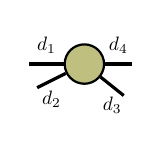
\begin{tikzpicture}[baseline=-0.5ex]
    \tikzset{tensor/.style = {minimum size = 0.5cm,shape = circle,thick,draw=black,inner sep = 0pt}, edge/.style = {thick,line width=.4mm},every loop/.style={}}
    \def\x{6}
    \def\y{0}
     \node[tensor,fill=green!50!red!50!white] (B) at (\x+1,\y) {$\Tt$};
    \draw[edge] (B) -- (\x+0.3,0) node [midway,above] {\scalebox{0.7}{\dimcolor{$d_1$}}};
    \draw[edge] (B) -- (\x+1.6,0) node [midway,above] {\scalebox{0.7}{\dimcolor{$d_4$}}};
    \draw[edge] (B) -- (\x+0.4,-0.3) node [midway, below] {\scalebox{0.7}{\dimcolor{$d_2$}}};
    \draw[edge] (B) -- (\x+1.5,-0.4)node [midway, below] {\scalebox{0.7}{\dimcolor{$d_3$}}};
\end{tikzpicture}
=
\begin{tikzpicture}[baseline=\baseline]
    \tikzset{tensor/.style = {minimum size = 0.5cm,shape = circle,thick,draw=black,inner sep = 0pt}, edge/.style   = {thick,line width=.4mm},every loop/.style={}}
    \def\y{0}
    \def\x{0}
  \node[tensor,fill=red!30!white] (D) at (\x-1,\y){$\Gt_1$};
  \node[tensor,fill=red!50!white] (A) at (\x,\y){\scalebox{0.85}{$\Gt_2$}};
  \node[tensor,fill=blue!50!white] (B) at (\x+1,\y){$\Gt_3$};
   \node[tensor,fill=blue!20!white] (C) at (\x+2,\y){$\Gt_4$};
    \draw[edge](A) -- (\x,\y-0.7)node [midway,left] {\edgelabel{$d_2$}};
    \draw[edge](B) -- (\x+1,\y-0.7)node [midway,left] {\edgelabel{$d_3$}};
    \draw[edge](C) -- (\x+2,\y-0.7)node [midway,left] {\edgelabel{$d_4$}};
     \draw[edge](D) -- (\x-1,\y-0.7)node [midway,left] {\edgelabel{$d_1$}};
    \draw[edge](D) -- (A) node [midway,above] {\edgelabel{$R_1$}};
    \draw[edge](A) -- (B) node [midway,above] {\edgelabel{$R_2$}};
    \draw[edge](B) -- (C) node [midway,above] {\edgelabel{$R_3$}};
\end{tikzpicture}.
\end{center}

Since $\Tt$ represents a probability distribution, its entries must be non-negative and sum to one.
In the context of machine learning, where we want to optimize the core tensors with respect to some loss function~(e.g. log-likelihood), there are several constraints one can impose on the core tensors $\Gt_1,\cdots,\Gt_N$ to ensure these two properties. 
One easy way to ensure non-negativity of the entries of $\Tt$ is to constrain the core tensors to have non-negative entries, or to apply a non-negative valued "activation" function component-wise to all the core tensors' entries. Another way, with its roots in quantum physics, is to assume that the entries of $\Tt$ are the square roots of the probabilities, rather than the probabilities themselves: $\Tt_{i_1,\cdots,i_N} = \sqrt{\PP(X_1=i_1,\cdots,X_N=i_N)}$. When $\Tt$ is in the TT format, this corresponds to the following tensor network:
$$
\PP(X_1=i_1,\cdots,X_4=i_4) = (\Tt_{i_1,\cdots,i_4})^2 = 
\begin{tikzpicture}[baseline=\baseline]
    \tikzset{tensor/.style = {minimum size = 0.5cm,shape = circle,thick,draw=black,inner sep = 0pt}, edge/.style   = {thick,line width=.4mm},every loop/.style={}}
    \def\y{-0.35}
    \def\x{0}
  \node[tensor,fill=red!30!white] (D) at (\x-1,\y){$\Gt_1$};
  \node[tensor,fill=red!50!white] (A) at (\x,\y){\scalebox{0.85}{$\Gt_2$}};
  \node[tensor,fill=blue!50!white] (B) at (\x+1,\y){$\Gt_3$};
   \node[tensor,fill=blue!20!white] (C) at (\x+2,\y){$\Gt_4$};
   \node[tensor,fill=red!30!white] (G1) at (\x-1,\y+0.85){$\Gt_1$};
  \node[tensor,fill=red!50!white] (G2) at (\x,\y+0.85){\scalebox{0.85}{$\Gt_2$}};
  \node[tensor,fill=blue!50!white] (G3) at (\x+1,\y+0.85){$\Gt_3$};
   \node[tensor,fill=blue!20!white] (G4) at (\x+2,\y+0.85){$\Gt_4$};
    \draw[edge](G1) -- (\x-1,\y+1.65)node [very near end, above]{\scalebox{0.7} {\indcolor{$i_1$}}};
    \draw[edge](G2) -- (\x,\y+1.65)node [very near end, above]{\scalebox{0.7} {\indcolor{$i_2$}}};
    \draw[edge](G3) -- (\x+1,\y+1.65)node [very near end, above]{\scalebox{0.7}{\indcolor{$i_3$}}};
    \draw[edge](G4) -- (\x+2,\y+1.65)node [very near end, above]{\scalebox{0.7}{\indcolor{$i_4$}}};
    \draw[edge](G1) -- (G2)node [midway,above] {\edgelabel{$R_1$}};
    \draw[edge](G2) -- (G3)node [midway,above] {\edgelabel{$R_2$}};
    \draw[edge](G3) -- (G4)node [midway,above] {\edgelabel{$R_3$}};
    \draw[edge](A) -- (\x,\y-0.7)node [very near end, below] {\scalebox{0.7}{\indcolor{$i_2$}}};
    \draw[edge](B) -- (\x+1,\y-0.7)node [very near end, below]{\scalebox{0.7} {\indcolor{$i_3$}}};
    \draw[edge](C) -- (\x+2,\y-0.7)node [very near end, below] {\scalebox{0.7}{\indcolor{$i_4$}}};
     \draw[edge](D) -- (\x-1,\y-0.7)node [very near end, below] {\scalebox{0.7}{\indcolor{$i_1$}}};
    \draw[edge](D) -- (A) node [midway,above] {\edgelabel{$R_1$}};
    \draw[edge](A) -- (B) node [midway,above] {\edgelabel{$R_2$}};
    \draw[edge](B) -- (C) node [midway,above] {\edgelabel{$R_3$}};
\end{tikzpicture}
.
$$

Using the copy tensor, we can write this as:
\begin{align}\label{eqn:parametrized-prob}
    \PP(X_1,\cdots,X_4) \simeq
    \begin{tikzpicture}[baseline=\baseline]
    \tikzset{tensor/.style = {minimum size = 0.5cm,shape = circle,thick,draw=black,inner sep = 0pt}, edge/.style   = {thick,line width=.4mm},every loop/.style={}}
    \def\y{-0.35}
    \def\x{0}
  \node[tensor,fill=red!30!white] (D) at (\x-1,\y-0.25){$\Gt_1$};
  \node[tensor,fill=red!50!white] (A) at (\x,\y-0.25){\scalebox{0.85}{$\Gt_2$}};
  \node[tensor,fill=blue!50!white] (B) at (\x+1,\y-0.25){$\Gt_3$};
   \node[tensor,fill=blue!20!white] (C) at (\x+2,\y-0.25){$\Gt_4$};
   \node[tensor,fill=red!30!white] (G1) at (\x-1,\y+1){$\Gt_1$};
  \node[tensor,fill=red!50!white] (G2) at (\x,\y+1){\scalebox{0.85}{$\Gt_2$}};
  \node[tensor,fill=blue!50!white] (G3) at (\x+1,\y+1){$\Gt_3$};
   \node[tensor,fill=blue!20!white] (G4) at (\x+2,\y+1){$\Gt_4$};
    \draw[edge](G1) -- (G2)node [midway,above] {\edgelabel{$R_1$}};
    \draw[edge](G2) -- (G3)node [midway,above] {\edgelabel{$R_2$}};
    \draw[edge](G3) -- (G4)node [midway,above] {\edgelabel{$R_3$}};
    \draw[edge](D) -- (A) node [midway,above] {\edgelabel{$R_1$}};
    \draw[edge](A) -- (B) node [midway,above] {\edgelabel{$R_2$}};
    \draw[edge](B) -- (C) node [midway,above] {\edgelabel{$R_3$}};
    \draw  node[fill = black,circle,inner sep=0pt,minimum size=4pt] (m_1) at (\x-1,\y+0.35) {};
    \draw  node[fill = black,circle,inner sep=0pt,minimum size=4pt] (m_2) at (\x,\y+0.35) {};
    \draw  node[fill = black,circle,inner sep=0pt,minimum size=4pt] (m_3) at (\x+1,\y+0.35) {};
    \draw  node[fill = black,circle,inner sep=0pt,minimum size=4pt] (m_4) at (\x+2,\y+0.35) {};
    \draw[edge](D)--(G1);
    \draw[edge](A)--(G2);
    \draw[edge](B)--(G3);    \draw[edge](C)--(G4);
    \draw[edge](m_1) -- (\x-1.35,\y+0.35);
    \draw[edge](m_4) -- (\x+2.35,\y+0.35);
    \draw[edge](m_2) -- (\x-0.35,\y+0.35);
    \draw[edge](m_3) -- (\x+1.35,\y+0.35);
\end{tikzpicture}
\end{align}

To ensure that the probabilities sum to one, we can choose to model un-normalized squared-root probabilities, since, as we will see, computing the normalization constant is very easy when the probability tensor is in the TT format. We thus assume that
$$\PP(X_1=i_1,\cdots,X_N=i_N) = \frac{(\Tt_{i_1,\cdots,i_N})^2}{\zeta},$$
where $\zeta = \sum_{i_1,\cdots,i_N}(\Tt_{i_1,\cdots,i_N})^2$ is the normalization constant. Similarly to efficient operations in the TT format presented in Section~\ref{sec:efficient-operations}, this normalization factor can be efficiently computed in the TT format: 
$$\zeta= \sum_{i_1,\cdots,i_4}\Tt_{i_1,\cdots,i_4}^2
=
\begin{tikzpicture}[baseline=\baseline]
    \tikzset{tensor/.style = {minimum size = 0.5cm,shape = circle,thick,draw=black,inner sep = 0pt}, edge/.style   = {thick,line width=.4mm},every loop/.style={}}
    \def\y{-0.35}
    \def\x{0}
  \node[tensor,fill=red!30!white] (D) at (\x-1,\y-0.25){$\Gt_1$};
  \node[tensor,fill=red!50!white] (A) at (\x,\y-0.25){\scalebox{0.85}{$\Gt_2$}};
    \node[tensor,fill=blue!50!white] (B) at (\x+1,\y-0.25){$\Gt_3$};
    \node[tensor,fill=blue!20!white] (C) at (\x+2,\y-0.25){$\Gt_4$};
     \node[tensor,fill=red!30!white] (G1) at (\x-1,\y+1){$\Gt_1$};
    \node[tensor,fill=red!50!white] (G2) at (\x,\y+1){\scalebox{0.85}{$\Gt_2$}};
    \node[tensor,fill=blue!50!white] (G3) at (\x+1,\y+1){$\Gt_3$};
    \node[tensor,fill=blue!20!white] (G4) at (\x+2,\y+1){$\Gt_4$};

    \draw[edge](G1) -- (G2)node [midway,above] {\edgelabel{$R_1$}};
    \draw[edge](G2) -- (G3)node [midway,above] {\edgelabel{$R_2$}};
    \draw[edge](G3) -- (G4)node [midway,above] {\edgelabel{$R_3$}};
    \draw[edge](D) -- (A) node [midway,above] {\edgelabel{$R_1$}};
    \draw[edge](A) -- (B) node [midway,above] {\edgelabel{$R_2$}};
    \draw[edge](B) -- (C) node [midway,above] {\edgelabel{$R_3$}};
    \draw[edge](G1)--(D);
    \draw[edge](G2)--(A);
    \draw[edge](G3)--(B);
    \draw[edge](G4)--(C);
\end{tikzpicture}.
$$
The idea above is also called \emph{Born Machine}~\citep{glasser2019expressive,han2018unsupervised}.
Similarly to what we showed in Section~\ref{sub:probs}, we can compute marginal distributions of TT parametrized probability distributions~(see Eq.~\eqref{eqn:parametrized-prob}) as tensor networks:
\begin{enumerate}
    \item %
    Using the law of total probabilities, the marginal distribution of $X_2,X_3$, and $X_4$ can be expressed as 
    \begin{align*}
    \PP(X_2=i_2, X_3=i_3, X_4=i_4) 
    &= \sum_{i_1=1}^{d_1}\PP(X_1=i_1,\cdots,X_4=i_4)\\ 
    &=
    \begin{tikzpicture}[baseline=\baseline]
    \tikzset{tensor/.style = {minimum size = 0.5cm,shape = circle,thick,draw=black,inner sep = 0pt}, edge/.style   = {thick,line width=.4mm},every loop/.style={}}
    \def\y{-0.35}
    \def\x{0}
  \node[tensor,fill=red!30!white] (D) at (\x-1,\y-0.25){$\Gt_1$};
  \node[tensor,fill=red!50!white] (A) at (\x,\y-0.25){\scalebox{0.85}{$\Gt_2$}};
  \node[tensor,fill=blue!50!white] (B) at (\x+1,\y-0.25){$\Gt_3$};
   \node[tensor,fill=blue!20!white] (C) at (\x+2,\y-0.25){$\Gt_4$};
   \node[tensor,fill=red!30!white] (G1) at (\x-1,\y+1){$\Gt_1$};
  \node[tensor,fill=red!50!white] (G2) at (\x,\y+1){\scalebox{0.85}{$\Gt_2$}};
  \node[tensor,fill=blue!50!white] (G3) at (\x+1,\y+1){$\Gt_3$};
   \node[tensor,fill=blue!20!white] (G4) at (\x+2,\y+1){$\Gt_4$};
    \draw[edge](G1) -- (G2)node [midway,above] {\edgelabel{$R_1$}};
    \draw[edge](G2) -- (G3)node [midway,above] {\edgelabel{$R_2$}};
    \draw[edge](G3) -- (G4)node [midway,above] {\edgelabel{$R_3$}};
    \draw[edge](D) -- (A) node [midway,above] {\edgelabel{$R_1$}};
    \draw[edge](A) -- (B) node [midway,above] {\edgelabel{$R_2$}};
    \draw[edge](B) -- (C) node [midway,above] {\edgelabel{$R_3$}};
    \draw  node[fill = black,circle,inner sep=0pt,minimum size=4pt] (m_1) at (\x-1,\y+0.35) {};
    \draw  node[fill = black,circle,inner sep=0pt,minimum size=4pt] (m_2) at (\x,\y+0.35) {};
    \draw  node[fill = black,circle,inner sep=0pt,minimum size=4pt] (m_3) at (\x+1,\y+0.35) {};
    \draw  node[fill = black,circle,inner sep=0pt,minimum size=4pt] (m_4) at (\x+2,\y+0.35) {};
    \draw[edge](D)--(G1);
    \draw[edge](A)--(G2);
    \draw[edge](B)--(G3);    \draw[edge](C)--(G4);
    \draw[edge](m_1) -- (\x-1.35,\y+0.35);
    \draw  node[fill = black,circle,inner sep=0pt,minimum size=4pt] (m) at (\x-1.35,\y+0.35) {};
    \draw[edge](m_4) -- (\x+2.35,\y+0.35) node [right] {\scalebox{0.7}{\indcolor{$i_4$}}};;
    \draw[edge](m_2) -- (\x-0.35,\y+0.35) node [left] {\scalebox{0.7}{\indcolor{$i_2$}}};;
    \draw[edge](m_3) -- (\x+1.35,\y+0.35) node [right] {\scalebox{0.7}{\indcolor{$i_3$}}};;
\end{tikzpicture}
=
\sum_{i_1}^{d_1}\Tt_{i_1,\cdots,i_4},
    \end{align*}
for all $i_2\in[d_1],i_3\in[d_3]$ and $i_4\in[d_4]$. 
\item We can similarly express the remaining marginal distributions. For example, the marginal distribution of $X_2$ can be written as
\begin{align*}
    \PP(X_2=i_2) 
    &= \sum_{i_1,i_3,i_4=1}^{d_1,d_3,d_4}\PP(X_1=i_1,\cdots,X_4=i_4)\\ 
    &=
    \begin{tikzpicture}[baseline=\baseline]
    \tikzset{tensor/.style = {minimum size = 0.5cm,shape = circle,thick,draw=black,inner sep = 0pt}, edge/.style   = {thick,line width=.4mm},every loop/.style={}}
    \def\y{-0.35}
    \def\x{0}
  \node[tensor,fill=red!30!white] (D) at (\x-1,\y-0.25){$\Gt_1$};
  \node[tensor,fill=red!50!white] (A) at (\x,\y-0.25){\scalebox{0.85}{$\Gt_2$}};
  \node[tensor,fill=blue!50!white] (B) at (\x+1,\y-0.25){$\Gt_3$};
   \node[tensor,fill=blue!20!white] (C) at (\x+2,\y-0.25){$\Gt_4$};
   \node[tensor,fill=red!30!white] (G1) at (\x-1,\y+1){$\Gt_1$};
  \node[tensor,fill=red!50!white] (G2) at (\x,\y+1){\scalebox{0.85}{$\Gt_2$}};
  \node[tensor,fill=blue!50!white] (G3) at (\x+1,\y+1){$\Gt_3$};
   \node[tensor,fill=blue!20!white] (G4) at (\x+2,\y+1){$\Gt_4$};
    \draw[edge](G1) -- (G2)node [midway,above] {\edgelabel{$R_1$}};
    \draw[edge](G2) -- (G3)node [midway,above] {\edgelabel{$R_2$}};
    \draw[edge](G3) -- (G4)node [midway,above] {\edgelabel{$R_3$}};
    \draw[edge](D) -- (A) node [midway,above] {\edgelabel{$R_1$}};
    \draw[edge](A) -- (B) node [midway,above] {\edgelabel{$R_2$}};
    \draw[edge](B) -- (C) node [midway,above] {\edgelabel{$R_3$}};
    \draw  node[fill = black,circle,inner sep=0pt,minimum size=4pt] (m_1) at (\x-1,\y+0.35) {};
    \draw  node[fill = black,circle,inner sep=0pt,minimum size=4pt] (m_2) at (\x,\y+0.35) {};
    \draw  node[fill = black,circle,inner sep=0pt,minimum size=4pt] (m_3) at (\x+1,\y+0.35) {};
    \draw  node[fill = black,circle,inner sep=0pt,minimum size=4pt] (m_4) at (\x+2,\y+0.35) {};
    \draw[edge](D)--(G1);
    \draw[edge](A)--(G2);
    \draw[edge](B)--(G3);    
    \draw[edge](C)--(G4);
    \draw[edge](m_1) -- (\x-1.35,\y+0.35);
    \draw  node[fill = black,circle,inner sep=0pt,minimum size=4pt] (m_5) at (\x-1.35,\y+0.35) {};
    \draw[edge](m_4) -- (\x+2.35,\y+0.35);
    \draw  node[fill = black,circle,inner sep=0pt,minimum size=4pt] (m_6) at (\x+2.35,\y+0.35) {};
    \draw[edge](m_2) -- (\x-0.35,\y+0.35) node [left] {\scalebox{0.7}{\indcolor{$i_2$}}};;
    \draw[edge](m_3) -- (\x+1.35,\y+0.35);
    \draw  node[fill = black,circle,inner sep=0pt,minimum size=4pt] (m_7) at (\x+1.35,\y+0.35) {};
\end{tikzpicture}
=
\sum_{i_1,i_3,i_4=1}^{d_1,d_3,d_4}\Tt_{i_1,\cdots,i_4},
    \end{align*}
\end{enumerate}
\subsection{Computing Expectations of Random Tensor Networks} 
We will now show how the tensor networks formalism can help us derive complex properties of random tensors. 
We begin this section by presenting two very useful propositions.
The first one is a trivial consequence of linearity of expectation, but will prove to be very useful in this section.
\begin{proposition}\label{prop:inner-expectation}
    Let $\At$ and $\Bt$ be two independent random tensor networks. tensor networks. Then their inner product in expectation is 
$$\EE\left(\begin{tikzpicture}[baseline=\baseline]
    \tikzset{tensor/.style = {minimum size = 0.5cm,shape = circle,thick,draw=black,inner sep = 0pt}, edge/.style = {thick,line width=.4mm},every loop/.style={}}
    \def\y{0}
    \def\x{0}
    \node[tensor,fill=red!50!blue!50!white] (At) at (\x,\y){\scalebox{0.85}{$\At$}};
    \node[tensor,fill=red!30!blue!50!white] (Bt) at (\x+1,\y){\scalebox{0.85}{$\Bt$}};
    \draw[edge] (At) -- (Bt);
    \draw[edge] (At) to [out=45,in=135] (Bt);
    \draw[edge] (At) to [out=-45,in=-135] (Bt);
    \draw[edge](At)--(\x-0.85,\y);
    \draw[edge](At)--(\x-0.75,\y+0.5);    \draw[edge](At)--(\x-0.75,\y-0.5);
    \draw[edge](Bt)--(\x+1.85,\y);
    \draw[edge](Bt)--(\x+1.75,\y+0.5);    \draw[edge](Bt)--(\x+1.75,\y-0.5);
\end{tikzpicture} \right)
=
\begin{tikzpicture}[baseline=\baseline]
    \tikzset{tensor/.style = {minimum size = 0.8cm,shape = circle,thick,draw=black,inner sep = 0pt}, edge/.style = {thick,line width=.4mm},every loop/.style={}}
    \def\y{0}
    \def\x{0}
    \node[tensor,fill=red!50!blue!50!white] (At) at (\x,\y){\scalebox{0.85}{$\EE(\At)$}};
    \node[tensor,fill=red!30!blue!50!white] (Bt) at (\x+1.5,\y){\scalebox{0.85}{$\EE(\Bt)$}};
    \draw[edge] (At) -- (Bt);
    \draw[edge] (At) to [out=45,in=135] (Bt);
    \draw[edge] (At) to [out=-45,in=-135] (Bt);
    \draw[edge](At)--(\x-0.85,\y);
    \draw[edge](At)--(\x-0.75,\y+0.5);    \draw[edge](At)--(\x-0.75,\y-0.5);
    \draw[edge](Bt)--(\x+2.35,\y);
    \draw[edge](Bt)--(\x+2.25,\y+0.5);    \draw[edge](Bt)--(\x+2.25,\y-0.5);
\end{tikzpicture}.
$$
\begin{proof}
The result directly follows from the linearity of the expected value and the independence of $\At$ and $\Bt$.
\end{proof}
\end{proposition}
The second one shows an interesting properties of matrices whose entries are drawn from a Gaussian distribution: the expectation of the outer product of such a matrix with itself reduces to a very simple tensor network. 
\begin{proposition}\label{prop:outer-prod}Let $\Ab\in\RR^{m\times n}$ be a random matrix whose elements are drawn identically and independently from the standard normal distribution. The expected value of the outer product of $\Ab$ with itself is 
$$\EE\left(
\begin{tikzpicture}[baseline=\baseline]
    \tikzset{tensor/.style = {minimum size = 0.5cm,shape = circle,thick,draw=black,inner sep = 0pt}, edge/.style = {thick,line width=.4mm},every loop/.style={}}
    \def\y{0.15}
    \def\x{0}
    \node[tensor,fill=green!50!blue!20!white] (A) at (\x,\y){\scalebox{0.85}{$\Ab$}};
    \node[tensor,fill=green!50!blue!20!white] (B) at (\x+1.5,\y){\scalebox{0.85}{$\Ab$}};
    \draw[edge](A) -- (\x-0.55,\y-0.55);
    \node[draw=none] () at (\x-0.5,\y-0.3) {\scalebox{0.7}{\dimcolor{$m$}}};
    \draw[edge](A) -- (\x+0.55,\y-0.55);
    \node[draw=none] () at (\x+0.5,\y-0.3) {\scalebox{0.7}{\dimcolor{$n$}}};
    \draw[edge](B) -- (\x+1,\y-0.55);
    \node[draw=none] () at (\x+1,\y-0.3) {\scalebox{0.7}{\dimcolor{$m$}}};
    \draw[edge](B) -- (\x+2,\y-0.55);
    \node[draw=none] () at (\x+2,\y-0.3) {\scalebox{0.7}{\dimcolor{$n$}}};
\end{tikzpicture}
\right)
=
\begin{tikzpicture}[baseline=\baseline]
    \tikzset{tensor/.style = {minimum size = 0.5cm,shape = circle,thick,draw=black,inner sep = 0pt}, edge/.style = {thick,line width=.4mm},every loop/.style={}}
    \def\y{0}
    \def\x{0}
    \draw[edge] (\x+0.15,\y-0.1) to [out=100,in=80] (\x+1.85,\y-0.1);
    \draw[edge] (\x+1.45,\y-0.1) to [out=100,in=80] (\x+3,\y-0.1);
    \node[draw=none] () at (\x+2.25,\y+0.5) {\scalebox{0.6}{\dimcolor{$n$}}};
    \node[draw=none] () at (\x+1,\y+0.5) {\scalebox{0.6}{\dimcolor{$m$}}};
\end{tikzpicture},
$$
where the right-hand side
is the outer product of two Kronecker delta~(i.e., $
\begin{tikzpicture}[baseline=\baseline]
    \tikzset{tensor/.style = {minimum size = 0.5cm,shape = circle,thick,draw=black,inner sep = 0pt}, edge/.style = {thick,line width=.4mm},every loop/.style={}}
    \def\y{0}
    \def\x{0}
    \draw[edge] (\x+0.15,\y-0.1) to [out=100,in=80] (\x+1.85,\y-0.1);
    \draw[edge] (\x+1.45,\y-0.1) to [out=100,in=80] (\x+3,\y-0.1);
    \node[draw=none] () at (\x+0.15,\y-0.25) {\scalebox{0.7}{\indcolor{$i_1$}}};
    \node[draw=none] () at (\x+3,\y-0.25) {\scalebox{0.7}{\indcolor{$i_4$}}};
    \node[draw=none] () at (\x+1.85,\y-0.25) {\scalebox{0.7}{\indcolor{$i_3$}}};
    \node[draw=none] () at (\x+1.45,\y-0.25) {\scalebox{0.7}{\indcolor{$i_2$}}};
\end{tikzpicture}
=\delta_{i_1i_3}\delta_{i_2i_4}$ for $i_1,i_3\in[m]$ and $i_2,i_4\in[n]$).
\begin{proof}
Since the entries of $\Ab$ are drawn independently from $\mathcal{N}(0,1)$, its vectorization follows a multivariate normal distribution, $\vectorize(\Ab) \sim \mathcal{N}(\mathbf{0},\Ib_{mn})$, and thus $\EE(\vectorize(\Ab)\vectorize(\Ab)^\ts) = \Ib_{mn}$. This means that 
$$ \EE(\Ab_{i_1i_2}\Ab_{i_3i_4})=
\begin{cases}
        1 & \text{ if } i_1=i_3\text{ and } i_2=i_4\\
        0 & \text{ otherwise, }
    \end{cases} 
    $$
hence, $\EE(\Ab\outprod\Ab)_{i_1i_2i_3i_4}=\EE(\Ab_{i_1i_2}\Ab_{i_3i_4}) = \delta_{i_1i_3}\delta_{i_2i_4}=
\begin{tikzpicture}[baseline=\baseline]
    \tikzset{tensor/.style = {minimum size = 0.5cm,shape = circle,thick,draw=black,inner sep = 0pt}, edge/.style = {thick,line width=.4mm},every loop/.style={}}
    \def\y{0}
    \def\x{0}
    \draw[edge] (\x+0.15,\y-0.1) to [out=100,in=80] (\x+1.85,\y-0.1);
    \draw[edge] (\x+1.45,\y-0.1) to [out=100,in=80] (\x+3,\y-0.1);
    \node[draw=none] () at (\x+0.15,\y-0.25) {\scalebox{0.7}{\indcolor{$i_1$}}};
    \node[draw=none] () at (\x+3,\y-0.25) {\scalebox{0.7}{\indcolor{$i_4$}}};
    \node[draw=none] () at (\x+1.85,\y-0.25) {\scalebox{0.7}{\indcolor{$i_3$}}};
    \node[draw=none] () at (\x+1.45,\y-0.25) {\scalebox{0.7}{\indcolor{$i_2$}}};
\end{tikzpicture}$, for all $i_1,i_3\in[m]$ and $i_2,i_4\in[n]$.


\end{proof}
\end{proposition}
\begin{remark}
    Note that different orderings of indices of $\EE(\Ab\outprod\Ab)$ lead to the following tensor networks:  
    \begin{align*}
            \EE(\Ab\outprod\Ab)_{i_1i_2i_4i_3}
            &= 
            \EE(\Ab_{i_1i_2}\Ab_{i_4i_3}) 
    = \delta_{i_1i_4}\delta_{i_2i_3}\\
    &=
    \begin{cases}
        1 & \text{ if } i_1=i_4\text{ and } i_2=i_3\\
        0 & \text{ otherwise, }
    \end{cases} 
    =
    \begin{tikzpicture}[baseline=\baseline]
    \tikzset{tensor/.style = {minimum size = 0.5cm,shape = circle,thick,draw=black,inner sep = 0pt}, edge/.style = {thick,line width=.4mm},every loop/.style={}}
    \def\y{0}
    \def\x{0}
    \draw[edge] (\x,\y-0.1) to [out=100,in=80] (\x+2,\y-0.1);
    \draw[edge] (\x+0.15,\y-0.1) to [out=100,in=80] (\x+1.85,\y-0.1);
    \node[draw=none] () at (\x,\y-0.25) {\scalebox{0.7}{\indcolor{$i_1$}}};
    \node[draw=none] () at (\x+2.15,\y-0.25) {\scalebox{0.7}{\indcolor{$i_4$}}};
    \node[draw=none] () at (\x+0.35,\y-0.25) {\scalebox{0.7}{\indcolor{$i_2$}}};
    \node[draw=none] () at (\x+1.7,\y-0.25) {\scalebox{0.7}{\indcolor{$i_3$}}};
\end{tikzpicture},
    \end{align*}
and
\begin{align*}
\EE(\Ab\outprod\Ab)_{i_1i_4i_2i_3} 
&= 
\EE(\Ab_{i_1i_4}\Ab_{i_2i_3})= \delta_{i_1i_2}\delta_{i_4i_3}\\
&=
\begin{cases}
        1 & \text{ if } i_1=i_2\text{ and } i_3=i_4\\
        0 & \text{ otherwise, }
\end{cases}
=
\begin{tikzpicture}[baseline=\baseline]
    \tikzset{tensor/.style = {minimum size = 0.5cm,shape = circle,thick,draw=black,inner sep = 0pt}, edge/.style = {thick,line width=.4mm},every loop/.style={}}
    \def\y{0}
    \def\x{0}
    \draw[edge] (\x+0.15,\y-0.1) to [out=100,in=80] (\x+1.85,\y-0.1);
    \draw[edge] (\x+2,\y-0.1) to [out=100,in=80] (\x+3.65,\y-0.1);
    \node[draw=none] () at (\x+0.15,\y-0.25) {\scalebox{0.7}{\indcolor{$i_1$}}};
    \node[draw=none] () at (\x+1.85,\y-0.25) {\scalebox{0.7}{\indcolor{$i_2$}}};
    \node[draw=none] () at (\x+2.15,\y-0.25) {\scalebox{0.7}{\indcolor{$i_3$}}};
    \node[draw=none] () at (\x+3.65,\y-0.25) {\scalebox{0.7}{\indcolor{$i_4$}}};
\end{tikzpicture}.
\end{align*}
\end{remark}
Next, we show how Propositions~\ref{prop:inner-expectation} and~\ref{prop:outer-prod} can be used to derive a very simple tensor network derivation of the expected value of the product of a random matrix with Gaussian entries with itself. 
\begin{proposition}\label{prop:wishart-mean}
If $\Ab\in\RR^{m\times n}$ is a random matrix whose elements are drawn i.i.d from the standard normal distribution, then $\EE(\Ab^\ts\Ab) = m\Ib_n$. 
\begin{proof}
        Using Propositions~\ref{prop:inner-expectation} and~\ref{prop:outer-prod} we can write 
\begin{align*}
\EE(\Ab^\ts\Ab) 
&= 
\EE\left(\begin{tikzpicture}[baseline=\baseline]
    \tikzset{tensor/.style = {minimum size = 0.5cm,shape = circle,thick,draw=black,inner sep = 0pt}, edge/.style = {thick,line width=.4mm},every loop/.style={}}
    \def\y{0}
    \def\x{0}
    \node[tensor,fill=red!30!blue!30!white] (A1) at (\x,\y){\scalebox{0.85}{$\Ab$}};
    \node[tensor,fill=red!30!blue!30!white] (A2) at (\x+1,\y){\scalebox{0.85}{$\Ab$}};
    \draw[edge](A1) -- (A2) node [midway, above]{\scalebox{0.7}{\dimcolor{$m$}}};
    \draw[edge](A1) -- (\x-0.85,\y) node [midway, above]{\scalebox{0.7}{\dimcolor{$n$}}};
    \draw[edge](A2) -- (\x+1.85,\y) node [midway, above]{\scalebox{0.7}{\dimcolor{$n$}}};
\end{tikzpicture}\right)
=
\EE\left(\begin{tikzpicture}[baseline=\baseline]
    \tikzset{tensor/.style = {minimum size = 0.5cm,shape = circle,thick,draw=black,inner sep = 0pt}, edge/.style = {thick,line width=.4mm},every loop/.style={}}
    \def\y{0}
    \def\x{0}
    \node[tensor,fill=red!30!blue!30!white] (A2) at (\x,\y-0.5){\scalebox{0.85}{$\Ab$}};
    \node[tensor,fill=red!30!blue!30!white] (A1) at (\x,\y+0.5){\scalebox{0.85}{$\Ab$}};
    \draw[edge](\x+0.25,\y+0.4) -- (\x+1.25,\y+0.4) -- (\x+1.25,\y-0.4) -- (\x+0.25,\y-0.4);
    \draw[edge](\x+0.2,\y+0.65)--(\x+1.25,\y+0.65)node [midway, above]{\scalebox{0.7}{\dimcolor{$n$}}};
    \draw[edge](\x+0.2,\y-0.65)--(\x+1.25,\y-0.65)node [midway, below]{\scalebox{0.7}{\dimcolor{$n$}}};
    \node[draw=none] () at (\x+1.45,\y) {\scalebox{0.7}{\dimcolor{$m$}}};
    \draw[dotted](\x+0.55,\y+1)--(\x+0.55,\y-1);
\end{tikzpicture}\right)\\
\ \
&\textequal{Prop.~\ref{prop:inner-expectation}}
\ \
\begin{tikzpicture}[baseline=\baseline]
   \tikzset{tensor/.style = {minimum size = 0.5cm,shape = circle,thick,draw=black,inner sep = 0pt}, edge/.style = {thick,line width=.4mm},every loop/.style={}}
    \def\y{0}
    \def\x{0}
    \node[tensor,fill=red!30!blue!30!white] (A1) at (\x,\y+0.5){\scalebox{0.85}{$\Ab$}};
    \node[tensor,fill=red!30!blue!30!white] (A2) at (\x,\y-0.5){\scalebox{0.85}{$\Ab$}};
    \draw[edge,draw=blue](\x+0.25,\y+0.4) -- (\x+1.65,\y+0.4);
    \draw[edge, draw=red](\x+1.65,\y+0.4)-- (\x+1.95,\y+0.4) -- (\x+1.95,\y-0.4)--(\x+1.65,\y+0-0.4);
    \draw[edge, draw=blue](\x+1.65,\y-0.4) -- (\x+0.25,\y-0.4);
    \draw[edge, draw=blue](\x+0.2,\y+0.65)--(\x+1.95,\y+0.65)node [midway, above]{\scalebox{0.7}{\dimcolor{$n$}}};
    \draw[edge,draw=blue](\x+0.2,\y-0.65)--(\x+1.95,\y-0.65)node [midway, below]{\scalebox{0.7}{\dimcolor{$n$}}};
    \node[draw=none] () at (\x+2.15,\y) {\scalebox{0.7}{\dimcolor{$m$}}};
    \node at (\x-0.55,\y) {$\EE\left( \vphantom{\rule{0pt}{1cm}} \right.$};
    \node at (\x+0.55,\y) {$\left. \vphantom{\rule{0pt}{1cm}} \right)$};
    \node at (\x+1.15,\y) {$\EE\left( \vphantom{\rule{0pt}{1cm}} \right.$};
    \node at (\x+2.35,\y) {$\left. \vphantom{\rule{0pt}{1cm}} \right)$};
\end{tikzpicture}
~~\textequal{Prop.~\ref{prop:outer-prod}}
\ \ 
\begin{tikzpicture}[baseline=\baseline]
   \tikzset{tensor/.style = {minimum size = 0.5cm,shape = circle,thick,draw=black,inner sep = 0pt}, edge/.style = {thick,line width=.4mm},every loop/.style={}}
    \def\y{0}
    \def\x{0}
    \draw[edge,draw=blue](\x+1.35,\y+0.4) -- (\x+1.65,\y+0.4);
    \draw[edge, draw=red](\x+1.65,\y+0.4)-- (\x+1.95,\y+0.4) -- (\x+1.95,\y-0.4)--(\x+1.65,\y+0-0.4);
    \draw[edge, draw=blue](\x+1.35,\y-0.4) -- (\x+1.65,\y-0.4);
    \draw[edge, draw=blue](\x+1.35,\y-0.4) -- (\x+1.35,\y-0.4);
    \draw[edge, draw=blue](\x+1.35,\y+0.65)--(\x+1.95,\y+0.65);
    \draw[edge,draw=blue](\x+1.35,\y-0.65)--(\x+1.95,\y-0.65);
    \node[draw=none] () at (\x+2.15,\y) {\scalebox{0.7}{\dimcolor{$m$}}};
    \node[draw=none] () at (\x+1.35,\y) {\scalebox{0.7}{\dimcolor{$m$}}};
    \node[draw=none] () at (\x+0.85,\y) {\scalebox{0.7}{\dimcolor{$n$}}};
    \draw[edge, draw=blue](\x+1.35,\y+0.65)to[out=170,in=190](\x+1.35,\y-0.65);
    \draw[edge, draw=blue](\x+1.35,\y+0.4)to[out=190,in=170](\x+1.35,\y-0.4);
\end{tikzpicture}
= m\Ib_n.
\end{align*}
The final diagram is obtained by contracting the legs of size $m$. As observed, once the contraction is performed, the resulting expression is simply the trace of the identity matrix, which corresponds to the circle of size $m$ in the above equality.
\end{proof}
\end{proposition}
The previous proposition can be interpreted as a statement on the mean of a Wishart distribution.  
Recall that  sampling a matrix $\mat X$ from the Wishart distribution $W_p(\mat \Sigma, m)$, where $\mat \Sigma \in \RR^{n\times n}$ is a covariance matrix, is done by sampling each column of a matrix $\mat A\in\mathbb R^{m\times n}$ from the multivariate normal $\mathcal N(\vec 0 , \mat \Sigma)$ independently and setting $\mat X = \mat A^\top\mat A$. Hence, the matrix $\Ab ^\top \Ab$ in Proposition~\ref{prop:inner-expectation} follows the Wishart distribution  $W_p(\mat I,m)$.
\begin{remark} As a consequence of Proposition~\ref{prop:inner-expectation}, if $\Ab \in \RR^{m \times n}$ is a random matrix with entries drawn from the standard normal distribution, then $\EE(\norm{\Ab}_F^2) = mn$. 
This result can be extended to higher-order tensors whose entries are drawn i.i.d. from the standard normal distribution, e.g., if $\Tt\in\RR^{d_1\times d_2\times\cdots\times d_N}$ then $\EE(\norm{\Tt}_F^2) = d_1d_2\cdots d_N$.
\end{remark}
By leveraging the properties of random Gaussian matrices established in the previous propositions, we can compute the expected norm of their product. Once again, the proof is remarkably simple when expressed through tensor networks, whereas an explicit treatment using indices and summations would be considerably more intricate.
\begin{proposition}\label{prop:expected-norm}
    Let $\Ab\in\RR^{m\times r}$ and $\Bb\in\RR^{r\times n}$ be random matrices whose entries are independently and identically distributed (i.i.d.) according to the standard normal distribution with mean zero and variance one. Then, the expected value of the squared Frobenius norm of their product is given by $\EE({\norm{\Ab\Bb}^2_F}) = mnr$.
\begin{proof}
Using Proposition~\ref{prop:inner-expectation} we can write
\begin{align*}
 \EE({\norm{\Ab\Bb}^2_F})
 &= 
 \EE\left(\begin{tikzpicture}[baseline=\baseline]
   \tikzset{tensor/.style = {minimum size = 0.5cm,shape = circle,thick,draw=black,inner sep = 0pt}, edge/.style = {thick,line width=.4mm},every loop/.style={}}
    \def\y{0}
    \def\x{0}
    \node[tensor,fill=red!50!white] (A) at (\x,\y+0.5){\scalebox{0.85}{$\Ab$}};
    \node[tensor,fill=blue!50!white] (B) at (\x+1,\y+0.5){\scalebox{0.85}{$\Bb$}};
    \draw[edge] (A) -- (B) node [midway,above]{\scalebox{0.7}{\dimcolor{$r$}}};
    \node[tensor,fill=red!50!white] (A1) at (\x,\y-0.5){\scalebox{0.85}{$\Ab$}};
    \node[tensor,fill=blue!50!white] (B1) at (\x+1,\y-0.5){\scalebox{0.85}{$\Bb$}};
    \draw[edge] (A1) -- (B1) node [midway,above]{\scalebox{0.7}{\dimcolor{$r$}}};
    \draw[edge] (A) to [out=-150,in=160, distance=0.5cm] (A1);
    \draw[edge] (B) to [out=-30,in=20, distance=0.5cm] (B1);
    \node[draw=none] () at (\x-0.75,\y) {\scalebox{0.7}{\dimcolor{$m$}}};
    \node[draw=none] () at (\x+1.75,\y) {\scalebox{0.7}{\dimcolor{$n$}}};
    \end{tikzpicture}\right)\\
&=
\EE\left(\begin{tikzpicture}[baseline=\baseline]
   \tikzset{tensor/.style = {minimum size = 0.5cm,shape = circle,thick,draw=black,inner sep = 0pt}, edge/.style = {thick,line width=.4mm},every loop/.style={}}
    \def\y{0.25}
    \def\x{0}
    \node[tensor,fill=red!50!white] (A) at (\x,\y){\scalebox{0.85}{$\Ab$}}; 
    \node[tensor,fill=red!50!white] (A1) at (\x+1,\y){\scalebox{0.85}{$\Ab$}};
    \draw[edge](A)--(A1)node[midway,above] {\scalebox{0.7}{\dimcolor{$m$}}};
    \draw[edge](A)--(\x,\y-0.85)node[midway,left] {\scalebox{0.7}{\dimcolor{$r$}}};
    \draw[edge](A1)--(\x+1,\y-0.85)node[midway,right] {\scalebox{0.7}{\dimcolor{$r$}}};
    \node[tensor,fill=blue!50!white] (B) at (\x+2,\y){\scalebox{0.85}{$\Bb$}}; 
    \node[tensor,fill=blue!50!white] (B1) at (\x+3,\y){\scalebox{0.85}{$\Bb$}};
    \draw[edge](B)--(B1)node[midway,above] {\scalebox{0.7}{\dimcolor{$n$}}};
    \draw[edge](B)--(\x+2,\y-0.85)node[midway,left] {\scalebox{0.7}{\dimcolor{$r$}}};
    \draw[edge](B1)--(\x+3,\y-0.85)node[midway,right] {\scalebox{0.7}{\dimcolor{$r$}}};
    \draw[edge](\x+2,\y-0.85) -- (\x+2,\y-1) -- (\x+1,\y-1) -- (\x+1,\y-0.85);
    \draw[edge](\x+3,\y-0.85) -- (\x+3,\y-1.25) -- (\x,\y-1.25) -- (\x,\y-0.85);
    \draw[dotted](\x+1.5,\y+0.5) -- (\x+1.5,\y-1.65);
\end{tikzpicture}\right)
=
\begin{tikzpicture}[baseline=\baseline]
   \tikzset{tensor/.style = {minimum size = 0.5cm,shape = circle,thick,draw=black,inner sep = 0pt}, edge/.style = {thick,line width=.4mm},every loop/.style={}}
    \def\y{0}
    \def\x{0}
    \node[tensor,fill=red!50!white] (A) at (\x,\y){\scalebox{0.85}{$\Ab$}}; 
    \node[tensor,fill=red!50!white] (A1) at (\x+1,\y){\scalebox{0.85}{$\Ab$}};
    \draw[edge, draw=red](A)--(A1)node[midway,above] {\scalebox{0.7}{\dimcolor{$m$}}};
   \node[tensor,fill=blue!50!white] (B) at (\x+2,\y){\scalebox{0.85}{$\Bb$}}; 
    \node[tensor,fill=blue!50!white] (B1) at (\x+3,\y){\scalebox{0.85}{$\Bb$}};
    \draw[edge, draw=blue](B)--(B1)node[midway,above] {\scalebox{0.7}{\dimcolor{$n$}}};
    \node at (\x-0.55,\y) {$\EE\Biggl ( $};
    \node (eq) at (\x+1.39,\y) {$\Biggr )\EE$};
    \node (eq) at (\x+1.73,\y) {$\Biggl($};
    \draw[edge, draw=blue](B) -- (\x+2,\y-0.85);
    \draw[edge, draw=blue](B1) -- (\x+3,\y-0.85);
    \draw[edge, draw=red](A) -- (\x,\y-0.85);
    \draw[edge, draw=red](A1) -- (\x+1,\y-0.85);
    \draw[edge](\x+1,\y-0.85) -- (\x+1,\y-1) -- (\x+2,\y-1)--(\x+2,\y-0.85);
    \draw[edge](\x+3,\y-0.85) -- (\x+3,\y-1.2) -- (\x,\y-1.2) -- (\x,\y-0.85);
    \node[draw=none] () at (\x+1.65,\y-0.85) {\scalebox{0.7}{\dimcolor{$r$}}};
    \node[draw=none] () at (\x+0.5,\y-0.95) {\scalebox{0.7}{\dimcolor{$r$}}};
\end{tikzpicture}\Biggr).
\end{align*}
By Proposition~\ref{prop:wishart-mean}, we have $\EE\left(\begin{tikzpicture}[baseline=\baseline]
   \tikzset{tensor/.style = {minimum size = 0.5cm,shape = circle,thick,draw=black,inner sep = 0pt}, edge/.style = {thick,line width=.4mm},every loop/.style={}}
    \def\y{0.15}
    \def\x{0}
    \node[tensor,fill=red!50!white] (A) at (\x,\y){\scalebox{0.85}{$\Ab$}}; 
    \node[tensor,fill=red!50!white] (A1) at (\x+1,\y){\scalebox{0.85}{$\Ab$}};
    \draw[edge, draw=red](A)--(A1)node[midway,above] {\scalebox{0.7}{\dimcolor{$m$}}};
    \draw[edge, draw=red](A) -- (\x,\y-0.85)node[midway,left] {\scalebox{0.7}{\dimcolor{$r$}}};
    \draw[edge, draw=red](A1) -- (\x+1,\y-0.85)node[midway,right] {\scalebox{0.7}{\dimcolor{$r$}}};
\end{tikzpicture}\right)
=
m\begin{tikzpicture}[baseline=\baseline]
   \tikzset{tensor/.style = {minimum size = 0.5cm,shape = circle,thick,draw=black,inner sep = 0pt}, edge/.style = {thick,line width=.4mm},every loop/.style={}}
    \def\y{0}
    \def\x{0}
     \draw[edge, draw=red] (\x,\y-0.1) to [out=100,in=80] (\x+2,\y-0.1);
    \node[draw=none] () at (\x+1,\y+0.65) {\scalebox{0.7}{\dimcolor{$r$}}};
\end{tikzpicture}$
and 
$\EE\left(\begin{tikzpicture}[baseline=\baseline]
   \tikzset{tensor/.style = {minimum size = 0.5cm,shape = circle,thick,draw=black,inner sep = 0pt}, edge/.style = {thick,line width=.4mm},every loop/.style={}}
    \def\y{0.15}
    \def\x{0}
    \node[tensor,fill=blue!50!white] (B) at (\x,\y){\scalebox{0.85}{$\Bb$}}; 
    \node[tensor,fill=blue!50!white] (B1) at (\x+1,\y){\scalebox{0.85}{$\Bb$}};
    \draw[edge, draw=blue](B)--(B1)node[midway,above] {\scalebox{0.7}{\dimcolor{$n$}}};
    \draw[edge, draw=blue](B) -- (\x,\y-0.85)node[midway,left] {\scalebox{0.7}{\dimcolor{$r$}}};
    \draw[edge, draw=blue](B1) -- (\x+1,\y-0.85)node[midway,right] {\scalebox{0.7}{\dimcolor{$r$}}};
\end{tikzpicture}\right)
= 
n\begin{tikzpicture}[baseline=\baseline]
   \tikzset{tensor/.style = {minimum size = 0.5cm,shape = circle,thick,draw=black,inner sep = 0pt}, edge/.style = {thick,line width=.4mm},every loop/.style={}}
    \def\y{0}
    \def\x{0}
     \draw[edge, draw=blue] (\x,\y-0.1) to [out=100,in=80] (\x+2,\y-0.1);
    \node[draw=none] () at (\x+1,\y+0.65) {\scalebox{0.7}{\dimcolor{$r$}}};
\end{tikzpicture}.
$ 
Since there are contractions between the legs of size $r$ we finally obtain
\begin{align*}
 \EE({\norm{\Ab\Bb}^2_F})
 = 
 \EE\left(\begin{tikzpicture}[baseline=\baseline]
   \tikzset{tensor/.style = {minimum size = 0.5cm,shape = circle,thick,draw=black,inner sep = 0pt}, edge/.style = {thick,line width=.4mm},every loop/.style={}}
    \def\y{0}
    \def\x{0}
    \node[tensor,fill=red!50!white] (A) at (\x,\y+0.5){\scalebox{0.85}{$\Ab$}};
    \node[tensor,fill=blue!50!white] (B) at (\x+1,\y+0.5){\scalebox{0.85}{$\Bb$}};
    \draw[edge] (A) -- (B) node [midway,above]{\scalebox{0.7}{\dimcolor{$r$}}};
    \node[tensor,fill=red!50!white] (A1) at (\x,\y-0.5){\scalebox{0.85}{$\Ab$}};
    \node[tensor,fill=blue!50!white] (B1) at (\x+1,\y-0.5){\scalebox{0.85}{$\Bb$}};
    \draw[edge] (A1) -- (B1) node [midway,above]{\scalebox{0.7}{\dimcolor{$r$}}};
    \draw[edge] (A) to [out=-150,in=160, distance=0.5cm] (A1);
    \draw[edge] (B) to [out=-30,in=20, distance=0.5cm] (B1);
    \node[draw=none] () at (\x-0.75,\y) {\scalebox{0.7}{\dimcolor{$m$}}};
    \node[draw=none] () at (\x+1.75,\y) {\scalebox{0.7}{\dimcolor{$n$}}};
    \end{tikzpicture}\right)
=
mn\  \begin{tikzpicture}     [baseline=\baseline]
 \tikzset{tensor/.style = {minimum size = 0.5cm,shape = circle,thick,draw=black,inner sep = 0pt}, edge/.style = {thick,line 
width=.4mm},every loop/.style={}}
    \def\y{0}
    \def\x{1}
    \draw[edge](\x+2,\y) -- (\x+2,\y-0.35) -- (\x+3,\y-0.35)--(\x+3,\y);
    \draw[edge](\x+1,\y) -- (\x+1,\y-0.5) -- (\x+4,\y-0.5) -- (\x+4,\y);
    \draw[edge, draw=red] (\x+2,\y) to [out=100,in=80](\x+1,\y);
    \draw[edge, draw=blue] (\x+3,\y) to [out=100,in=80](\x+4,\y);
    \node[draw=none] () at (\x+2.5,\y-0.65) {\scalebox{0.7}{\dimcolor{$r$}}};
    \node[draw=none] () at (\x+3.5,\y+0.5) {\scalebox{0.7}{\dimcolor{$r$}}};
    \node[draw=none] () at (\x+1.5,\y+0.5) {\scalebox{0.7}{\dimcolor{$r$}}};
\end{tikzpicture}
= mnr.
\end{align*}
\end{proof}
\end{proposition}
Now that we understand how to compute the expected norm of products of Gaussian random matrices, we can extend this method to evaluate expectations of more complex tensor networks.

\paragraph{Example} Suppose, we have an arbitrary tensor network, e.g.,
$$\Tt = 
\begin{tikzpicture}[baseline=\baseline]
   \tikzset{tensor/.style = {minimum size = 0.5cm,shape = circle,thick,draw=black,inner sep = 0pt}, edge/.style = {thick,line width=.4mm},every loop/.style={}}
    \def\y{0}
    \def\x{0}
    \node[tensor,fill=red!20!blue!20!white] (A) at (\x,\y){\scalebox{0.85}{$\At$}}; 
    \node[tensor,fill=red!40!blue!20!white] (B) at (\x+1,\y){\scalebox{0.85}{$\Bt$}};
    \node[tensor,fill=red!40!blue!30!white] (C) at (\x+2,\y){\scalebox{0.85}{$\Ct$}};
    \node[tensor,fill=red!60!blue!40!white] (G) at (\x+1,\y+1){\scalebox{0.85}{$\Gt$}};
    \draw[edge](A)--(B)node[midway,above] {\scalebox{0.7}{\dimcolor{$r_1$}}};
    \draw[edge](B)--(C)node[midway,above] {\scalebox{0.7}{\dimcolor{$r_2$}}};
    \draw[edge](G)--(A)node[midway,left] {\scalebox{0.7}{\dimcolor{$d_1$}}};
    \draw[edge](G)--(B)node[midway,left] {\scalebox{0.7}{\dimcolor{$d_2$}}};
    \draw[edge](G)--(C)node[midway,right] {\scalebox{0.7}{\dimcolor{$d_3$}}};
    \draw[edge](A)--(\x,\y-0.85)node[midway,left] {\scalebox{0.7}{\dimcolor{$m_1$}}};
    \draw[edge](B)--(\x+1,\y-0.85)node[midway,left] {\scalebox{0.7}{\dimcolor{$m_2$}}};
    \draw[edge](C)--(\x+2,\y-0.85)node[midway,left] {\scalebox{0.7}{\dimcolor{$m_3$}}};
\end{tikzpicture},
$$
where $\At\in\RR^{m_1\times d_1\times r_1}, \Bt\in\RR^{m_2\times r_1\times d_2\times r_2}, \Ct\in\RR^{m_3\times r_2\times d_3}$ and $\Gt\in\RR^{d_1\times d_2\times d_3}$ are tensors whose elements are drawn i.i.d. from the standard normal distribution, and we want to compute the expectation of $\norm{\Tt}^2_F$. Using tensor network diagrams, we have
\begin{align*}
    \EE\left(\norm{\begin{tikzpicture}[baseline=\baseline]
   \tikzset{tensor/.style = {minimum size = 0.5cm,shape = circle,thick,draw=black,inner sep = 0pt}, edge/.style = {thick,line width=.4mm},every loop/.style={}}
    \def\y{0}
    \def\x{0}
    \node[tensor,fill=red!20!blue!20!white] (A) at (\x,\y){\scalebox{0.85}{$\At$}}; 
    \node[tensor,fill=red!40!blue!20!white] (B) at (\x+1,\y){\scalebox{0.85}{$\Bt$}};
    \node[tensor,fill=red!40!blue!30!white] (C) at (\x+2,\y){\scalebox{0.85}{$\Ct$}};
    \node[tensor,fill=red!60!blue!40!white] (G) at (\x+1,\y+1){\scalebox{0.85}{$\Gt$}};
    \draw[edge](A)--(B)node[midway,above] {\scalebox{0.7}{\dimcolor{$r_1$}}};
    \draw[edge](B)--(C)node[midway,above] {\scalebox{0.7}{\dimcolor{$r_2$}}};
    \draw[edge](G)--(A)node[midway,left] {\scalebox{0.7}{\dimcolor{$d_1$}}};
    \draw[edge](G)--(B)node[midway,left] {\scalebox{0.7}{\dimcolor{$d_2$}}};
    \draw[edge](G)--(C)node[midway,right] {\scalebox{0.7}{\dimcolor{$d_3$}}};
    \draw[edge](A)--(\x,\y-0.85)node[midway,left] {\scalebox{0.7}{\dimcolor{$m_1$}}};
    \draw[edge](B)--(\x+1,\y-0.85)node[midway,left] {\scalebox{0.7}{\dimcolor{$m_2$}}};
    \draw[edge](C)--(\x+2,\y-0.85)node[midway,left] {\scalebox{0.7}{\dimcolor{$m_3$}}};
\end{tikzpicture}}_F^2\right)
=
\EE\left(\begin{tikzpicture}[baseline=\baseline]
   \tikzset{tensor/.style = {minimum size = 0.5cm,shape = circle,thick,draw=black,inner sep = 0pt}, edge/.style = {thick,line width=.4mm},every loop/.style={}}
    \def\y{0.5}
    \def\x{0}
    \node[tensor,fill=red!20!blue!20!white] (A_1) at (\x,\y){\scalebox{0.85}{$\At$}}; 
    \node[tensor,fill=red!40!blue!20!white] (B_1) at (\x+1,\y){\scalebox{0.85}{$\Bt$}};
    \node[tensor,fill=red!40!blue!30!white] (C_1) at (\x+2,\y){\scalebox{0.85}{$\Ct$}};
    \node[tensor,fill=red!60!blue!40!white] (G_1) at (\x+1,\y+1){\scalebox{0.85}{$\Gt$}};
    \draw[edge](A_1)--(B_1)node[midway,above] {\scalebox{0.7}{\dimcolor{$r_1$}}};
    \draw[edge](B_1)--(C_1)node[midway,above] {\scalebox{0.7}{\dimcolor{$r_2$}}};
    \draw[edge](G_1)--(A_1)node[midway,left] {\scalebox{0.7}{\dimcolor{$d_1$}}};
    \draw[edge](G_1)--(B_1)node[midway,left] {\scalebox{0.7}{\dimcolor{$d_2$}}};
    \draw[edge](G_1)--(C_1)node[midway,right] {\scalebox{0.7}{\dimcolor{$d_3$}}};
    \node[tensor,fill=red!20!blue!20!white] (A) at (\x,\y-1){\scalebox{0.85}{$\At$}}; 
    \node[tensor,fill=red!40!blue!20!white] (B) at (\x+1,\y-1){\scalebox{0.85}{$\Bt$}};
    \node[tensor,fill=red!40!blue!30!white] (C) at (\x+2,\y-1){\scalebox{0.85}{$\Ct$}};
    \node[tensor,fill=red!60!blue!40!white] (G) at (\x+1,\y-2){\scalebox{0.85}{$\Gt$}};
    \draw[edge](A)--(B)node[midway,above] {\scalebox{0.7}{\dimcolor{$r_1$}}};
    \draw[edge](B)--(C)node[midway,above] {\scalebox{0.7}{\dimcolor{$r_2$}}};
    \draw[edge](G)--(A)node[midway,left] {\scalebox{0.7}{\dimcolor{$d_1$}}};
    \draw[edge](G)--(B)node[midway,left] {\scalebox{0.7}{\dimcolor{$d_2$}}};
    \draw[edge](G)--(C)node[midway,right] {\scalebox{0.7}{\dimcolor{$d_3$}}};
    \draw[edge](A_1)--(A)node[midway,left] {\scalebox{0.7}{\dimcolor{$m_1$}}};
    \draw[edge](B_1)--(B)node[midway,left] {\scalebox{0.7}{\dimcolor{$m_2$}}};
    \draw[edge](C_1)--(C)node[midway,left] {\scalebox{0.7}{\dimcolor{$m_3$}}};
\end{tikzpicture}\right).
\end{align*}
From Prop.~\ref{prop:wishart-mean}, we know that 

$$
\EE\left(\begin{tikzpicture}[baseline=\baseline]
   \tikzset{tensor/.style = {minimum size = 0.5cm,shape = circle,thick,draw=black,inner sep = 0pt}, edge/.style = {thick,line width=.4mm},every loop/.style={}}
    \def\y{0.5}
    \def\x{0}
    \node[tensor,fill=red!20!blue!20!white] (A1) at (\x,\y){\scalebox{0.85}{$\At$}}; 
    \node[tensor,fill=red!20!blue!20!white] (A2) at (\x,\y-1){\scalebox{0.85}{$\At$}}; 
    \draw[edge, draw=blue](A1) -- (A2)node [midway,right]{\scalebox{0.7}{\dimcolor{$m_1$}}};
    \draw[edge, draw=blue](A1) -- (\x+0.65,\y)node [midway,above]{\scalebox{0.7}{\dimcolor{$r_1$}}};
    \draw[edge, draw=blue](A2) -- (\x+0.65,\y-1)node [midway,above]{\scalebox{0.7}{\dimcolor{$r_1$}}};
    \draw[edge,draw=blue](A1) -- (\x,\y+0.65)node [midway,right]{\scalebox{0.7}{\dimcolor{$d_1$}}};
    \draw[edge,draw=blue](A2) -- (\x,\y-1.65)node [midway,right]{\scalebox{0.7}{\dimcolor{$d_1$}}};
\end{tikzpicture}\right) = m_1
\begin{tikzpicture}[baseline=\baseline]
   \tikzset{tensor/.style = {minimum size = 0.5cm,shape = circle,thick,draw=black,inner sep = 0pt}, edge/.style = {thick,line width=.4mm},every loop/.style={}}
    \def\y{0}
    \def\x{0}
    \draw[edge, draw=blue](\x-0.65,\y+0.5) -- (\x-0.65,\y-0.5);
    \draw[edge, draw=blue](\x,\y+0.5) to [out=190,in=170] (\x,\y-0.5);
    \node[draw=none] () at (\x-0.8,\y) {\scalebox{0.7}{\dimcolor{$d_1$}}};
    \node[draw=none] () at (\x-0.1,\y) {\scalebox{0.7}{\dimcolor{$r_1$}}};
\end{tikzpicture},\  
\EE\left(\begin{tikzpicture}[baseline=\baseline]
   \tikzset{tensor/.style = {minimum size = 0.5cm,shape = circle,thick,draw=black,inner sep = 0pt}, edge/.style = {thick,line width=.4mm},every loop/.style={}}
    \def\y{0.5}
    \def\x{0}
    \node[tensor,fill=red!40!blue!20!white] (B1) at (\x,\y){\scalebox{0.85}{$\Bt$}};
    \node[tensor,fill=red!40!blue!20!white] (B2) at (\x,\y-1){\scalebox{0.85}{$\Bt$}};
    \draw[edge, draw=red](B1) -- (B2)node [midway,right]{\scalebox{0.7}{\dimcolor{$m_2$}}};
    \draw[edge, draw=red](B1) -- (\x,\y+0.65)node [midway,right]{\scalebox{0.7}{\dimcolor{$d_2$}}};
    \draw[edge, draw=red](B1) -- (\x+0.65,\y)node [midway,above]{\scalebox{0.7}{\dimcolor{$r_2$}}};
    \draw[edge, draw=red](B2) -- (\x+0.65,\y-1)node [midway,above]{\scalebox{0.7}{\dimcolor{$r_2$}}};
    \draw[edge, draw=red](B1) -- (\x-0.65,\y)node [midway,above]{\scalebox{0.7}{\dimcolor{$r_1$}}};
    \draw[edge, draw=red](B2) -- (\x-0.65,\y-1)node [midway,above]{\scalebox{0.7}{\dimcolor{$r_1$}}};
     \draw[edge, draw=red](B2) --(\x,\y-1.65)node [midway,right]{\scalebox{0.7}{\dimcolor{$d_2$}}};
    \end{tikzpicture}\right)
    =
m_2
\begin{tikzpicture}[baseline=\baseline]
   \tikzset{tensor/.style = {minimum size = 0.5cm,shape = circle,thick,draw=black,inner sep = 0pt}, edge/.style = {thick,line width=.4mm},every loop/.style={}}
    \def\y{0}
    \def\x{0}
    \draw[edge, draw=red](\x-0.65,\y+0.5) -- (\x-0.65,\y-0.5);
    \draw[edge, draw=red](\x,\y+0.5) to [out=190,in=170] (\x,\y-0.5);
    \draw[edge, draw=red](\x-1.3,\y+0.5) to [out=-20,in=-5] (\x-1.3,\y-0.5);
    \node[draw=none] () at (\x-0.8,\y) {\scalebox{0.7}{\dimcolor{$d_2$}}};
    0.5);
    \node[draw=none] () at (\x-1.2,\y) {\scalebox{0.7}{\dimcolor{$r_1$}}};
    \node[draw=none] () at (\x-0.1,\y) {\scalebox{0.7}{\dimcolor{$r_2$}}};
\end{tikzpicture}
\text{ and }
    \EE\left(\begin{tikzpicture}[baseline=\baseline]
   \tikzset{tensor/.style = {minimum size = 0.5cm,shape = circle,thick,draw=black,inner sep = 0pt}, edge/.style = {thick,line width=.4mm},every loop/.style={}}
    \def\y{0.5}
    \def\x{0}
    \node[tensor,fill=red!40!blue!30!white] (C1) at (\x,\y){\scalebox{0.85}{$\Ct$}};
    \node[tensor,fill=red!40!blue!30!white] (C2) at (\x,\y-1){\scalebox{0.85}{$\Ct$}};
    \draw[edge, draw=orange](C1) -- (C2)node [midway,right]{\scalebox{0.7}{\dimcolor{$m_3$}}};
    \draw[edge, draw=orange](C1) -- (\x,\y+0.65)node [midway,right]{\scalebox{0.7}{\dimcolor{$d_3$}}};
    \draw[edge, draw=orange](C1) -- (\x-0.65,\y)node [midway,above]{\scalebox{0.7}{\dimcolor{$r_2$}}};
    \draw[edge, draw=orange](C2) -- (\x-0.65,\y-1)node [midway,above]{\scalebox{0.7}{\dimcolor{$r_2$}}};
     \draw[edge, draw=orange](C2) --(\x,\y-1.65)node [midway,right]{\scalebox{0.7}{\dimcolor{$d_3$}}};
    \end{tikzpicture}\right)
=
m_3
\begin{tikzpicture}[baseline=\baseline]
   \tikzset{tensor/.style = {minimum size = 0.5cm,shape = circle,thick,draw=black,inner sep = 0pt}, edge/.style = {thick,line width=.4mm},every loop/.style={}}
    \def\y{0}
    \def\x{0}
    \draw[edge, draw=orange](\x-0.65,\y+0.5) -- (\x-0.65,\y-0.5);
    \draw[edge, draw=orange](\x-1.3,\y+0.5) to [out=-20,in=-5] (\x-1.3,\y-0.5);
    \node[draw=none] () at (\x-0.8,\y) {\scalebox{0.7}{\dimcolor{$d_3$}}};
    0.5);
    \node[draw=none] () at (\x-1.2,\y) {\scalebox{0.7}{\dimcolor{$r_2$}}};
\end{tikzpicture},
$$
and thus by Proposition~\ref{prop:inner-expectation} we can write:
\begin{align*}
\EE\left(\begin{tikzpicture}[baseline=\baseline]
   \tikzset{tensor/.style = {minimum size = 0.5cm,shape = circle,thick,draw=black,inner sep = 0pt}, edge/.style = {thick,line width=.4mm},every loop/.style={}}
    \def\y{0.5}
    \def\x{0}
    \node[tensor,fill=red!20!blue!20!white] (A_1) at (\x,\y){\scalebox{0.85}{$\At$}}; 
    \node[tensor,fill=red!40!blue!20!white] (B_1) at (\x+1,\y){\scalebox{0.85}{$\Bt$}};
    \node[tensor,fill=red!40!blue!30!white] (C_1) at (\x+2,\y){\scalebox{0.85}{$\Ct$}};
    \draw[edge](A_1)--(B_1)node[midway,above] {\scalebox{0.7}{\dimcolor{$r_1$}}};
    \draw[edge](B_1)--(C_1)node[midway,above] {\scalebox{0.7}{\dimcolor{$r_2$}}};
    \draw[edge](A_1) -- (\x+0.65,\y+0.65) node[midway,left] {\scalebox{0.7}{\dimcolor{$d_1$}}};
    \draw[edge](B_1) -- (\x+1,\y+0.65) node[midway,right] {\scalebox{0.7}{\dimcolor{$d_2$}}};
    \draw[edge](C_1) -- (\x+1.65,\y+0.65) node[midway,right] {\scalebox{0.7}{\dimcolor{$d_3$}}};  \node[tensor,fill=red!20!blue!20!white] (A) at (\x,\y-1){\scalebox{0.85}{$\At$}}; 
    \node[tensor,fill=red!40!blue!20!white] (B) at (\x+1,\y-1){\scalebox{0.85}{$\Bt$}};
    \node[tensor,fill=red!40!blue!30!white] (C) at (\x+2,\y-1){\scalebox{0.85}{$\Ct$}};
    \draw[edge](A)--(B) node[midway,above] {\scalebox{0.7}{\dimcolor{$r_1$}}};
    \draw[edge](B)--(C)node[midway,above] {\scalebox{0.7}{\dimcolor{$r_2$}}};
    \draw[edge](A_1)--(A) node[midway,left] {\scalebox{0.7}{\dimcolor{$m_1$}}};
    \draw[edge](B_1)--(B) node[midway,left] {\scalebox{0.7}{\dimcolor{$m_2$}}};
    \draw[edge](C_1)--(C) node[midway,left] {\scalebox{0.7}{\dimcolor{$m_3$}}};
    \draw[edge](A) -- (\x+0.65,\y-1.65)node[midway,left] {\scalebox{0.7}{\dimcolor{$d_1$}}};
    \draw[edge](B) -- (\x+1,\y-1.65)node[midway,right] {\scalebox{0.7}{\dimcolor{$d_2$}}};
    \draw[edge](C) -- (\x+1.65,\y-1.65)node[midway,right] {\scalebox{0.7}{\dimcolor{$d_3$}}};
\end{tikzpicture}\right)
&=
\begin{tikzpicture}[baseline=\baseline]
   \tikzset{tensor/.style = {minimum size = 0.5cm,shape = circle,thick,draw=black,inner sep = 0pt}, edge/.style = {thick,line width=.4mm},every loop/.style={}}
    \def\y{0.5}
    \def\x{0}
    \node[tensor,fill=red!20!blue!20!white] (A1) at (\x,\y){\scalebox{0.85}{$\At$}}; 
    \node[tensor,fill=red!20!blue!20!white] (A2) at (\x,\y-1){\scalebox{0.85}{$\At$}}; 
    \draw[edge, draw=blue](A1) -- (A2)node[midway,right] {\scalebox{0.7}{\dimcolor{$m_1$}}};
    \draw[edge, draw=blue](A1) -- (\x+0.65,\y)node[midway,above] {\scalebox{0.7}{\dimcolor{$r_1$}}};
    \draw[edge, draw=blue](A2) -- (\x+0.65,\y-1)node[midway,above] {\scalebox{0.7}{\dimcolor{$r_1$}}};
    \draw[edge,draw=blue](A1) -- (\x,\y+0.65)node[midway,right] {\scalebox{0.7}{\dimcolor{$d_1$}}};
    \draw[edge,draw=blue](A2) -- (\x,\y-1.65)node[midway,right] {\scalebox{0.7}{\dimcolor{$d_1$}}};
    \node at (\x-0.55,\y-0.5) {$\EE\left( \vphantom{\rule{0pt}{1cm}} \right.$};
    \node at (\x+1,\y-0.5) {$\left.\vphantom{\rule{0pt}{1cm}} \right)$};
    \node at (\x+1.45,\y-0.5){$\EE\left( \vphantom{\rule{0pt}{1cm}} \right.$};
    \node[tensor,fill=red!40!blue!20!white] (B1) at (\x+2,\y){\scalebox{0.85}{$\Bt$}};
    \node[tensor,fill=red!40!blue!20!white] (B2) at (\x+2,\y-1){\scalebox{0.85}{$\Bt$}};
    \draw[edge, draw=red](B1) -- (B2)node[midway,right] {\scalebox{0.7}{\dimcolor{$m_2$}}};
    \draw[edge, draw=red](B1) -- (\x+2.65,\y)node[midway,above] {\scalebox{0.7}{\dimcolor{$r_2$}}};
    \draw[edge, draw=red](B2) -- (\x+2.65,\y-1)node[midway,above] {\scalebox{0.7}{\dimcolor{$r_2$}}};
     \draw[edge, draw=red](B1) -- (\x+2,\y+0.65)node[midway,right] {\scalebox{0.7}{\dimcolor{$d_1$}}};
    \draw[edge, draw=red](B2) -- (\x+2,\y-1.65)node[midway,right] {\scalebox{0.7}{\dimcolor{$d_2$}}};
    \draw[edge, draw=red](B1) -- (\x+1.35,\y);
     \draw[edge, draw=red](B2) -- (\x+1.35,\y-1);
     \draw[edge](\x+1.35,\y) -- (\x+0.65,\y);
    \draw[edge](\x+1.35,\y-1) -- (\x+0.65,\y-1);
    \node at (\x+3,\y-0.5) {$\left.\vphantom{\rule{0pt}{1cm}} \right)$};
    \node at (\x+3.45,\y-0.5){$\EE\left( \vphantom{\rule{0pt}{1cm}} \right.$};
    \node[tensor,fill=red!40!blue!30!white] (C1) at (\x+4,\y){\scalebox{0.85}{$\Ct$}};
    \node[tensor,fill=red!40!blue!30!white] (C2) at (\x+4,\y-1){\scalebox{0.85}{$\Ct$}};
    \draw[edge, draw=orange](C1) -- (C2)node[midway,right] {\scalebox{0.7}{\dimcolor{$m_3$}}};
    \draw[edge, draw=orange](C1) -- (\x+3.25,\y);
     \draw[edge, draw=orange](C2) -- (\x+3.25,\y-1);
    \draw[edge, draw=orange](C1) --(\x+4,\y+0.65)node[midway,right] {\scalebox{0.7}{\dimcolor{$d_3$}}};
    \draw[edge, draw=orange](C2) -- (\x+4,\y-1.65)node[midway,right] {\scalebox{0.7}{\dimcolor{$d_3$}}};
    \draw[edge](\x+3.25,\y)--(\x+2.65,\y);
    \draw[edge](\x+3.25,\y-1)--(\x+2.65,\y-1);
    \node at (\x+4.5,\y-0.5) {$\left.\vphantom{\rule{0pt}{1cm}} \right)$};
\end{tikzpicture}\\
&= 
m_1m_2m_3
\begin{tikzpicture}[baseline=\baseline]
   \tikzset{tensor/.style = {minimum size = 0.5cm,shape = circle,thick,draw=black,inner sep = 0pt}, edge/.style = {thick,line width=.4mm},every loop/.style={}}
    \def\y{0}
    \def\x{0}
    \draw[edge, draw=blue](\x,\y+0.5) -- (\x,\y-0.5);
    \draw[edge, draw=blue](\x+0.5,\y+0.5) to [out=190,in=170] (\x+0.5,\y-0.5);
    \node[draw=none] () at (\x-0.15,\y) {\scalebox{0.7}{\dimcolor{$d_1$}}};
     \draw[edge, draw=red](\x+0.5,\y+0.5) to [out=-20,in=-5] (\x+0.5,\y-0.5);
    \node[draw=none] () at (\x+0.5,\y+0.65) {\scalebox{0.7}{\dimcolor{$r_1$}}};
    \node[draw=none] () at (\x+1.1,\y) {\scalebox{0.7}{\dimcolor{$d_2$}}};
    \draw[edge, draw=red](\x+1.25,\y+0.5) -- (\x+1.25,\y-0.5);
    \draw[edge, draw=red](\x+1.75,\y+0.5) to [out=190,in=170] (\x+1.75,\y-0.5);
    \draw[edge, draw=orange](\x+1.75,\y+0.5) to [out=-20,in=-5] (\x+1.75,\y-0.5);
    \node[draw=none] () at (\x+1.75,\y+0.65) {\scalebox{0.7}{\dimcolor{$r_2$}}};
    \draw[edge, draw=orange](\x+2.5,\y+0.5) -- (\x+2.5,\y-0.5);
    \node[draw=none] () at (\x+2.35,\y) {\scalebox{0.7}{\dimcolor{$d_3$}}};
  \end{tikzpicture}\\
&=
m_1m_2m_3r_1r_2
\begin{tikzpicture}[baseline=\baseline]
   \tikzset{tensor/.style = {minimum size = 0.5cm,shape = circle,thick,draw=black,inner sep = 0pt}, edge/.style = {thick,line width=.4mm},every loop/.style={}}
    \def\y{0}
    \def\x{0}
    \draw[edge, draw=blue](\x,\y+0.5) -- (\x,\y-0.5);
    \node[draw=none] () at (\x-0.15,\y) {\scalebox{0.7}{\dimcolor{$d_1$}}};
    \draw[edge, draw=red](\x+0.5,\y+0.5) -- (\x+0.5,\y-0.5);
    \node[draw=none] () at (\x+0.35,\y) {\scalebox{0.7}{\dimcolor{$d_2$}}};
    \draw[edge, draw=orange](\x+1,\y+0.5) -- (\x+1,\y-0.5);
    \node[draw=none] () at (\x+0.85,\y) {\scalebox{0.7}{\dimcolor{$d_3$}}};
\end{tikzpicture}.
\end{align*}
Therefore, since $\Gt$ is independent of $\At,\Bt$ and $\Ct$ we can use Proposition~\ref{prop:inner-expectation} again  and write 
\begin{align*}
    \EE\left(\begin{tikzpicture}[baseline=\baseline]
   \tikzset{tensor/.style = {minimum size = 0.5cm,shape = circle,thick,draw=black,inner sep = 0pt}, edge/.style = {thick,line width=.4mm},every loop/.style={}}
    \def\y{0.5}
    \def\x{0}
    \node[tensor,fill=red!20!blue!20!white] (A_1) at (\x,\y){\scalebox{0.85}{$\At$}}; 
    \node[tensor,fill=red!40!blue!20!white] (B_1) at (\x+1,\y){\scalebox{0.85}{$\Bt$}};
    \node[tensor,fill=red!40!blue!30!white] (C_1) at (\x+2,\y){\scalebox{0.85}{$\Ct$}};
    \node[tensor,fill=red!60!blue!40!white] (G_1) at (\x+1,\y+1){\scalebox{0.85}{$\Gt$}};
    \draw[edge](A_1)--(B_1)node[midway,above] {\scalebox{0.7}{\dimcolor{$r_1$}}};
    \draw[edge](B_1)--(C_1)node[midway,above] {\scalebox{0.7}{\dimcolor{$r_2$}}};
    \draw[edge](G_1)--(A_1)node[midway,left] {\scalebox{0.7}{\dimcolor{$d_1$}}};
    \draw[edge](G_1)--(B_1)node[midway,left] {\scalebox{0.7}{\dimcolor{$d_2$}}};
    \draw[edge](G_1)--(C_1)node[midway,right] {\scalebox{0.7}{\dimcolor{$d_3$}}};
    \node[tensor,fill=red!20!blue!20!white] (A) at (\x,\y-1){\scalebox{0.85}{$\At$}}; 
    \node[tensor,fill=red!40!blue!20!white] (B) at (\x+1,\y-1){\scalebox{0.85}{$\Bt$}};
    \node[tensor,fill=red!40!blue!30!white] (C) at (\x+2,\y-1){\scalebox{0.85}{$\Ct$}};
    \node[tensor,fill=red!60!blue!40!white] (G) at (\x+1,\y-2){\scalebox{0.85}{$\Gt$}};
    \draw[edge](A)--(B)node[midway,above] {\scalebox{0.7}{\dimcolor{$r_1$}}};
    \draw[edge](B)--(C)node[midway,above] {\scalebox{0.7}{\dimcolor{$r_2$}}};
    \draw[edge](G)--(A)node[midway,left] {\scalebox{0.7}{\dimcolor{$d_1$}}};
    \draw[edge](G)--(B)node[midway,left] {\scalebox{0.7}{\dimcolor{$d_2$}}};
    \draw[edge](G)--(C)node[midway,right] {\scalebox{0.7}{\dimcolor{$d_3$}}};
    \draw[edge](A_1)--(A)node[midway,left] {\scalebox{0.7}{\dimcolor{$m_1$}}};
    \draw[edge](B_1)--(B)node[midway,left] {\scalebox{0.7}{\dimcolor{$m_2$}}};
    \draw[edge](C_1)--(C)node[midway,left] {\scalebox{0.7}{\dimcolor{$m_3$}}};
\end{tikzpicture}\right)
&=
m_1m_2m_3r_1r_2
\EE\left(\begin{tikzpicture}[baseline=\baseline]
   \tikzset{tensor/.style = {minimum size = 0.5cm,shape = circle,thick,draw=black,inner sep = 0pt}, edge/.style = {thick,line width=.4mm},every loop/.style={}}
    \def\y{0.5}
    \def\x{0}
    \node[tensor,fill=red!60!blue!40!white] (G_1) at (\x+1,\y+1){\scalebox{0.85}{$\Gt$}};
    \node[tensor,fill=red!60!blue!40!white] (G) at (\x+1,\y-2){\scalebox{0.85}{$\Gt$}};
    \draw[edge](G_1)--(\x+1,\y+0.25);
    \draw[edge](G_1) -- (\x+0.5,\y+0.5);
    \draw[edge](G_1) -- (\x+1.5,\y+0.5);
    \draw[edge](G)--(\x+1,\y-1.25);
    \draw[edge](G)--(\x+0.5,\y-1.5);
    \draw[edge](G)--(\x+1.5,\y-1.5);
    \draw[edge, draw=blue](\x+0.5,\y+0.5)--(\x+0.5,\y-1.5)node[midway,left] {\scalebox{0.7}{\dimcolor{$d_1$}}};
    \draw[edge, draw=red](\x+1,\y+0.25)--(\x+1,\y-1.25)node[midway,right] {\scalebox{0.7}{\dimcolor{$d_2$}}};
     \draw[edge, draw=orange](\x+1.5,\y+0.5)--(\x+1.5,\y-1.5)node[midway,right] {\scalebox{0.7}{\dimcolor{$d_3$}}};
\end{tikzpicture}\right)
\ \ \ \textequal{Prop.~\ref{prop:wishart-mean}}\ \  m_1m_2m_3r_1r_2d_1d_2d_3.
\end{align*}
We can see how efficiently complex computations can be performed using tensor networks. We now introduce other identities involving random Gaussian matrices.
\begin{enumerate}
\item  The first identity is a useful consequence of \emph{Isserlis'} theorem~\citep{isserlis1918formula}.
\begin{theorem}\label{thm:isserlis}
Let $\ab\in\RR^{n}$ be a random vector whose elements are drawn i.i.d. from the normal distribution with mean zero and variance one. Then
\begin{align*}
\EE(\ab^{\outprod 4}) 
&= 
\EE\left(\begin{tikzpicture}[baseline=\baseline]
   \tikzset{tensor/.style = {minimum size = 0.5cm,shape = circle,thick,draw=black,inner sep = 0pt}, edge/.style = {thick,line width=.4mm},every loop/.style={}}
    \def\y{0.25}
    \def\x{0}
    \node[tensor,fill=red!20!blue!20!white] (a1) at (\x,\y){\scalebox{0.85}{$\ab$}}; 
    \node[tensor,fill=red!20!blue!20!white] (a2) at (\x+1,\y){\scalebox{0.85}{$\ab$}}; 
    \node[tensor,fill=red!20!blue!20!white] (a3) at (\x+2,\y){\scalebox{0.85}{$\ab$}}; 
    \node[tensor,fill=red!20!blue!20!white] (a4) at (\x+3,\y){\scalebox{0.85}{$\ab$}}; 
    \draw[edge](a1) -- (\x,\y-0.85);
    \draw[edge](a2) -- (\x+1,\y-0.85);
    \draw[edge](a3) -- (\x+2,\y-0.85);
    \draw[edge](a4) -- (\x+3,\y-0.85);
\end{tikzpicture}
\right)\\
&=
\begin{tikzpicture}[baseline=\baseline]
    \tikzset{tensor/.style = {minimum size = 0.5cm,shape = circle,thick,draw=black,inner sep = 0pt}, edge/.style = {thick,line width=.4mm},every loop/.style={}}
    \def\y{0}
    \def\x{0}
    \draw[edge] (\x+0.15,\y-0.1) to [out=100,in=80] (\x+1.85,\y-0.1);
    \draw[edge] (\x+2,\y-0.1) to [out=100,in=80] (\x+3.65,\y-0.1);
\end{tikzpicture}
+
\begin{tikzpicture}[baseline=\baseline]
    \tikzset{tensor/.style = {minimum size = 0.5cm,shape = circle,thick,draw=black,inner sep = 0pt}, edge/.style = {thick,line width=.4mm},every loop/.style={}}
    \def\y{0}
    \def\x{0}
    \draw[edge] (\x+0.15,\y-0.1) to [out=100,in=80] (\x+1.85,\y-0.1);
    \draw[edge] (\x+1.45,\y-0.1) to [out=100,in=80] (\x+3,\y-0.1);
\end{tikzpicture}
+
    \begin{tikzpicture}[baseline=\baseline]
    \tikzset{tensor/.style = {minimum size = 0.5cm,shape = circle,thick,draw=black,inner sep = 0pt}, edge/.style = {thick,line width=.4mm},every loop/.style={}}
    \def\y{0}
    \def\x{0}
    \draw[edge] (\x,\y-0.1) to [out=100,in=80] (\x+2,\y-0.1);
    \draw[edge] (\x+0.15,\y-0.1) to [out=100,in=80] (\x+1.85,\y-0.1);
\end{tikzpicture}
\end{align*}
where $\ab^{\outprod 4}$ denotes the outer product of $\ab$ with itself 4 times. In the last equality, each term in the sum corresponds to a different reshaping of the identity matrix.

This result can be extended to an arbitrary covariance structure: if $\ab$ is drawn from the multivariate normal $\mathcal N(\mathbf 0, \Sigmab )$, then
\begin{align*}
\EE(\ab^{\outprod 4})=
\begin{tikzpicture}[baseline=\baseline]
    \tikzset{tensor/.style = {minimum size = 0.4cm,shape = circle,thick,draw=black,inner sep = 0pt}, edge/.style = {thick,line width=.4mm},every loop/.style={}}
    \def\y{0}`
    \def\x{0}
    \draw[edge] (\x+0.15,\y-0.1) to [out=100,in=80] (\x+1.85,\y-0.1);
    \draw[edge] (\x+2,\y-0.1) to [out=100,in=80] (\x+3.65,\y-0.1);
    \node[tensor,fill=red!50!white] (A) at (\x+0.9,\y+0.35){\scalebox{0.85}{$\Sigmab$}};
    \node[tensor,fill=red!50!white] (A) at (\x+2.8,\y+0.35){\scalebox{0.85}{$\Sigmab$}};
\end{tikzpicture}
+
\begin{tikzpicture}[baseline=\baseline]
    \tikzset{tensor/.style = {minimum size = 0.4cm,shape = circle,thick,draw=black,inner sep = 0pt}, edge/.style = {thick,line width=.4mm},every loop/.style={}}
    \def\y{0}`
    \def\x{0}
    \draw[edge] (\x+0.15,\y-0.1) to [out=100,in=80] (\x+1.85,\y-0.1);
    \draw[edge] (\x+1.45,\y-0.1) to [out=100,in=80] (\x+3,\y-0.1);
    \node[tensor,fill=red!50!white] (A) at (\x+0.9,\y+0.35){\scalebox{0.85}{$\Sigmab$}};
    \node[tensor,fill=red!50!white] (A) at (\x+2.25,\y+0.35){\scalebox{0.85}{$\Sigmab$}};
\end{tikzpicture}
+
\begin{tikzpicture}[baseline=\baseline]
    \tikzset{tensor/.style = {minimum size = 0.4cm,shape = circle,thick,draw=black,inner sep = 0pt}, edge/.style = {thick,line width=.4mm},every loop/.style={}}
    \def\y{0.3}`
    \def\x{0}
    \draw[edge] (\x,\y-0.1) to [out=100,in=80] (\x+2,\y-0.1);
    \draw[edge] (\x+0.15,\y-0.45) to [out=100,in=80] (\x+1.85,\y-0.45);
    \node[tensor,fill=red!50!white] (A) at (\x+0.9,\y+0.45){\scalebox{0.85}{$\Sigmab$}};
    \node[tensor,fill=red!50!white] (A) at (\x+0.95,\y){\scalebox{0.85}{$\Sigmab$}};
\end{tikzpicture} .
\end{align*}


\begin{proof}
    We show the result for the case where the covariance is the identity. The proof extends straightforwardly to the case of an arbitrary covariance matrix. 
    
    Element-wise, by using Isserlis’
    theorem and using the fact that $\ab\sim\mathcal{N}(\mathbf{0},\Ib)$, for $i_1,\cdots,i_4\in[n]$, we have
\begin{align*}
(\EE(&\ab^{\outprod 4}))_{i_1,i_2,i_3,i_4} 
=
    \EE(\ab_{i_1}\ab_{i_2}\ab_{i_3}\ab_{i_4})\\
&= 
    \EE(\ab_{i_1}\ab_{i_2})\EE(\ab_{i_3}\ab_{i_4}) + \EE(\ab_{i_1}\ab_{i_3})\EE(\ab_{i_2}\ab_{i_4})
    +\EE(\ab_{i_1}\ab_{i_4})\EE(\ab_{i_2}\ab_{i_3})\\
&=
    \delta_{i_1i_2}\delta_{i_3i_4} + \delta_{i_1i_3}\delta_{i_2i_4} + \delta_{i_1i_4}\delta_{i_2i_3},
\end{align*}
which in tensor network notation gives:
\begin{align*}
\EE(\ab^{\outprod 4})_{i_1i_2i_3i_4}
=
\begin{tikzpicture}[baseline=\baseline]
    \tikzset{tensor/.style = {minimum size = 0.5cm,shape = circle,thick,draw=black,inner sep = 0pt}, edge/.style = {thick,line width=.4mm},every loop/.style={}}
    \def\y{0}
    \def\x{0}
    \draw[edge] (\x+0.15,\y-0.1) to [out=100,in=80] (\x+1.85,\y-0.1);
    \draw[edge] (\x+2,\y-0.1) to [out=100,in=80] (\x+3.65,\y-0.1);
    \node[draw=none] () at (\x+0.15,\y-0.25) {\scalebox{0.7}{\indcolor{$i_1$}}};
    \node[draw=none] () at (\x+1.85,\y-0.25) {\scalebox{0.7}{\indcolor{$i_2$}}};
    \node[draw=none] () at (\x+2.15,\y-0.25) {\scalebox{0.7}{\indcolor{$i_3$}}};
    \node[draw=none] () at (\x+3.65,\y-0.25) {\scalebox{0.7}{\indcolor{$i_4$}}};
\end{tikzpicture}
+
\begin{tikzpicture}[baseline=\baseline]
    \tikzset{tensor/.style = {minimum size = 0.5cm,shape = circle,thick,draw=black,inner sep = 0pt}, edge/.style = {thick,line width=.4mm},every loop/.style={}}
    \def\y{0}
    \def\x{0}
    \draw[edge] (\x+0.15,\y-0.1) to [out=100,in=80] (\x+1.85,\y-0.1);
    \draw[edge] (\x+1.45,\y-0.1) to [out=100,in=80] (\x+3,\y-0.1);
    \node[draw=none] () at (\x+0.15,\y-0.25) {\scalebox{0.7}{\indcolor{$i_1$}}};
    \node[draw=none] () at (\x+3,\y-0.25) {\scalebox{0.7}{\indcolor{$i_4$}}};
    \node[draw=none] () at (\x+1.85,\y-0.25) {\scalebox{0.7}{\indcolor{$i_3$}}};
    \node[draw=none] () at (\x+1.45,\y-0.25) {\scalebox{0.7}{\indcolor{$i_2$}}};
\end{tikzpicture}
+
    \begin{tikzpicture}[baseline=\baseline]
    \tikzset{tensor/.style = {minimum size = 0.5cm,shape = circle,thick,draw=black,inner sep = 0pt}, edge/.style = {thick,line width=.4mm},every loop/.style={}}
    \def\y{0}
    \def\x{0}
    \draw[edge] (\x,\y-0.1) to [out=100,in=80] (\x+2,\y-0.1);
    \draw[edge] (\x+0.15,\y-0.1) to [out=100,in=80] (\x+1.85,\y-0.1);
    \node[draw=none] () at (\x,\y-0.25) {\scalebox{0.7}{\indcolor{$i_1$}}};
    \node[draw=none] () at (\x+2.15,\y-0.25) {\scalebox{0.7}{\indcolor{$i_4$}}};
    \node[draw=none] () at (\x+0.35,\y-0.25) {\scalebox{0.7}{\indcolor{$i_2$}}};
    \node[draw=none] () at (\x+1.7,\y-0.25) {\scalebox{0.7}{\indcolor{$i_3$}}};
\end{tikzpicture}.
\end{align*}
\end{proof}
\end{theorem}
We can also extend the result of \emph{Isserlis' theorem} to the case where the random variable takes the form of a higher-order tensor. For example, for a third-order tensor $\At\in\RR^{d_1\times d_2\times d_3}$, we can write
\begin{align*}
    (\EE(\At^{\outprod 4}))_{i_1j_1r_1i_2j_2r_2i_3j_3r_3i_4j_4r_4}
&=\\
&\hspace{-3cm}\begin{tikzpicture}[baseline=\baseline]
    \tikzset{tensor/.style = {minimum size = 0.5cm,shape = circle,thick,draw=black,inner sep = 0pt}, edge/.style = {thick,line width=.4mm},every loop/.style={}}
    \def\x{0}
    \def\y{0}
    \draw[edge] (\x+0.15,\y-0.1) to [out=100,in=80] (\x+1.85,\y-0.1);
    \draw[edge] (\x+2,\y-0.1) to [out=100,in=80] (\x+3.65,\y-0.1);
    \node[draw=none] () at (\x+0.15,\y-0.25) {\scalebox{0.7}{\indcolor{$j_1$}}};
    \node[draw=none] () at (\x+1.85,\y-0.25) {\scalebox{0.7}{\indcolor{$j_2$}}};
    \node[draw=none] () at (\x+2.15,\y-0.25) {\scalebox{0.7}{\indcolor{$j_3$}}};
    \node[draw=none] () at (\x+3.65,\y-0.25) {\scalebox{0.7}{\indcolor{$j_4$}}};
    \draw[edge] (\x+0.15,\y+1) to [out=100,in=80] (\x+1.85,\y+1);
    \draw[edge] (\x+2,\y+1) to [out=100,in=80] (\x+3.65,\y+1);
    \node[draw=none] () at (\x+0.15,\y+0.9) {\scalebox{0.7}{\indcolor{$i_1$}}};
    \node[draw=none] () at (\x+1.85,\y+0.9) {\scalebox{0.7}{\indcolor{$i_2$}}};
    \node[draw=none] () at (\x+2.15,\y+0.9) {\scalebox{0.7}{\indcolor{$i_3$}}};
    \node[draw=none] () at (\x+3.65,\y+0.9) {\scalebox{0.7}{\indcolor{$i_4$}}};
    \draw[edge] (\x+0.15,\y-1) to [out=100,in=80] (\x+1.85,\y-1);
    \draw[edge] (\x+2,\y-1) to [out=100,in=80] (\x+3.65,\y-1);
    \node[draw=none] () at (\x+0.15,\y-1.15) {\scalebox{0.7}{\indcolor{$r_1$}}};
    \node[draw=none] () at (\x+1.85,\y-1.15) {\scalebox{0.7}{\indcolor{$r_2$}}};
    \node[draw=none] () at (\x+2.15,\y-1.15) {\scalebox{0.7}{\indcolor{$r_3$}}};
    \node[draw=none] () at (\x+3.65,\y-1.15) {\scalebox{0.7}{\indcolor{$r_4$}}};
\end{tikzpicture}
+
\begin{tikzpicture}[baseline=\baseline]
    \tikzset{tensor/.style = {minimum size = 0.5cm,shape = circle,thick,draw=black,inner sep = 0pt}, edge/.style = {thick,line width=.4mm},every loop/.style={}}
    \def\x{0}
    \def\y{0}
    \draw[edge] (\x+0.15,\y-0.1) to [out=100,in=80] (\x+1.85,\y-0.1);
    \draw[edge] (\x+1.45,\y-0.1) to [out=100,in=80] (\x+3,\y-0.1);
    \node[draw=none] () at (\x+0.15,\y-0.25) {\scalebox{0.7}{\indcolor{$j_1$}}};
    \node[draw=none] () at (\x+3,\y-0.25) {\scalebox{0.7}{\indcolor{$j_4$}}};
    \node[draw=none] () at (\x+1.85,\y-0.25) {\scalebox{0.7}{\indcolor{$j_3$}}};
    \node[draw=none] () at (\x+1.45,\y-0.25) {\scalebox{0.7}{\indcolor{$j_2$}}};
    \draw[edge] (\x+0.15,\y+1) to [out=100,in=80] (\x+1.85,\y+1);
    \draw[edge] (\x+1.45,\y+1) to [out=100,in=80] (\x+3,\y+1);
    \node[draw=none] () at (\x+0.15,\y+0.9) {\scalebox{0.7}{\indcolor{$i_1$}}};
    \node[draw=none] () at (\x+3,\y+0.9) {\scalebox{0.7}{\indcolor{$i_4$}}};
    \node[draw=none] () at (\x+1.85,\y+0.9) {\scalebox{0.7}{\indcolor{$i_3$}}};
    \node[draw=none] () at (\x+1.45,\y+0.9) {\scalebox{0.7}{\indcolor{$i_2$}}};
    \draw[edge] (\x+0.15,\y-1) to [out=100,in=80] (\x+1.85,\y-1);
    \draw[edge] (\x+1.45,\y-1) to [out=100,in=80] (\x+3,\y-1);
    \node[draw=none] () at (\x+0.15,\y-1.15) {\scalebox{0.7}{\indcolor{$r_1$}}};
    \node[draw=none] () at (\x+3,\y-1.15) {\scalebox{0.7}{\indcolor{$r_4$}}};
    \node[draw=none] () at (\x+1.85,\y-1.15) {\scalebox{0.7}{\indcolor{$r_3$}}};
    \node[draw=none] () at (\x+1.45,\y-1.15) {\scalebox{0.7}{\indcolor{$r_2$}}};
\end{tikzpicture}
+
    \begin{tikzpicture}[baseline=\baseline]
    \tikzset{tensor/.style = {minimum size = 0.5cm,shape = circle,thick,draw=black,inner sep = 0pt}, edge/.style = {thick,line width=.4mm},every loop/.style={}}
    \def\x{0}
    \def\y{0}
    \draw[edge] (\x,\y+1) to [out=100,in=80] (\x+2,\y+1);
    \draw[edge] (\x+0.15,\y+1) to [out=100,in=80] (\x+1.85,\y+1);
    \node[draw=none] () at (\x,\y+0.9) {\scalebox{0.7}{\indcolor{$i_1$}}};
    \node[draw=none] () at (\x+2.15,\y+0.9) {\scalebox{0.7}{\indcolor{$i_4$}}};
    \node[draw=none] () at (\x+0.35,\y+0.9) {\scalebox{0.7}{\indcolor{$i_2$}}};
    \node[draw=none] () at (\x+1.7,\y+0.9) {\scalebox{0.7}{\indcolor{$i_3$}}};
    \draw[edge] (\x,\y-0.1) to [out=100,in=80] (\x+2,\y-0.1);
    \draw[edge] (\x+0.15,\y-0.1) to [out=100,in=80] (\x+1.85,\y-0.1);
    \node[draw=none] () at (\x,\y-0.25) {\scalebox{0.7}{\indcolor{$j_1$}}};
    \node[draw=none] () at (\x+2.15,\y-0.25) {\scalebox{0.7}{\indcolor{$j_4$}}};
    \node[draw=none] () at (\x+0.35,\y-0.25) {\scalebox{0.7}{\indcolor{$j_2$}}};
    \node[draw=none] () at (\x+1.7,\y-0.25) {\scalebox{0.7}{\indcolor{$j_3$}}};
    \draw[edge] (\x,\y-1) to [out=100,in=80] (\x+2,\y-1);
    \draw[edge] (\x+0.15,\y-1) to [out=100,in=80] (\x+1.85,\y-1);
    \node[draw=none] () at (\x,\y-1.25) {\scalebox{0.7}{\indcolor{$r_1$}}};
    \node[draw=none] () at (\x+2.15,\y-1.25) {\scalebox{0.7}{\indcolor{$r_4$}}};
    \node[draw=none] () at (\x+0.35,\y-1.25) {\scalebox{0.7}{\indcolor{$r_2$}}};
    \node[draw=none] () at (\x+1.7,\y-1.25) {\scalebox{0.7}{\indcolor{$r_3$}}};
\end{tikzpicture},
\end{align*}
for $i_1,\cdots,i_4\in[d_1], j_1,\cdots,j_4\in [d_2]$ and $r_1,\cdots,r_4\in[d_3]$.
\item Using the above results, we can easily derive the expectation of  $(\Ab^\ts\Ab)^{\outprod 2}$ when $\Ab$ is a random matrix:
\begin{proposition}\label{prop:kronecker-exp}
    Let $\Ab\in\RR^{m\times n}$ be a random matrix whose elements are drawn i.i.d from the standard normal distribution. Then
\begin{align*}
\EE((\Ab^\ts\Ab)^{\outprod 2})) 
=
m^2\begin{tikzpicture}[baseline=\baseline]
    \tikzset{tensor/.style = {minimum size = 0.5cm,shape = circle,thick,draw=black,inner sep = 0pt}, edge/.style = {thick,line width=.4mm},every loop/.style={}}
    \def\y{0}
    \def\x{0}
    \draw[edge] (\x+0.15,\y-0.1) to [out=100,in=80] (\x+1.85,\y-0.1);
    \draw[edge] (\x+2,\y-0.1) to [out=100,in=80] (\x+3.65,\y-0.1);
    \node[draw=none] () at (\x+1,\y+0.5) {\scalebox{0.7}{\dimcolor{$n$}}};
    \node[draw=none] () at (\x+2.85,\y+0.5) {\scalebox{0.7}{\dimcolor{$n$}}};
\end{tikzpicture}
+m\begin{tikzpicture}[baseline=\baseline]
    \tikzset{tensor/.style = {minimum size = 0.5cm,shape = circle,thick,draw=black,inner sep = 0pt}, edge/.style = {thick,line width=.4mm},every loop/.style={}}
    \def\y{0}
    \def\x{0}
    \draw[edge] (\x+0.15,\y-0.1) to [out=100,in=80] (\x+1.85,\y-0.1);
    \draw[edge] (\x+1.45,\y-0.1) to [out=100,in=80] (\x+3,\y-0.1);
    \node[draw=none] () at (\x+1,\y+0.5) {\scalebox{0.7}{\dimcolor{$n$}}};
    \node[draw=none] () at (\x+2.25,\y+0.5) {\scalebox{0.7}{\dimcolor{$n$}}};
\end{tikzpicture}
+
m\begin{tikzpicture}[baseline=\baseline]
    \tikzset{tensor/.style = {minimum size = 0.5cm,shape = circle,thick,draw=black,inner sep = 0pt}, edge/.style = {thick,line width=.4mm},every loop/.style={}}
    \def\y{0}
    \def\x{0}
    \draw[edge] (\x,\y-0.1) to [out=100,in=80] (\x+2,\y-0.1);
    \draw[edge] (\x+0.15,\y-0.1) to [out=100,in=80] (\x+1.85,\y-0.1);
    \node[draw=none] () at (\x+1,\y+0.65) {\scalebox{0.7}{\dimcolor{$n$}}};
    \node[draw=none] () at (\x+1,\y+0.25) {\scalebox{0.7}{\dimcolor{$n$}}};
\end{tikzpicture}.
\end{align*}
\begin{proof}
By applying Theorem~\ref{thm:isserlis} to matrices and using Proposition~\ref{prop:wishart-mean}, we can derive the desired expression. First, from Theorem~\ref{thm:isserlis} we have
\begin{align*}
\EE(\Ab^{\outprod4})_{i_1j_1i_2j_2i_3j_3i_4j_4}
&= 
\EE\left(\begin{tikzpicture}[baseline=\baseline]
    \tikzset{tensor/.style = {minimum size = 0.5cm,shape = circle,thick,draw=black,inner sep = 0pt}, edge/.style = {thick,line width=.4mm},every loop/.style={}}
    \def\y{0.25}
    \def\x{0}
    \node[tensor,fill=green!50!blue!20!white] (A1) at (\x,\y){\scalebox{0.85}{$\Ab$}};
    \node[tensor,fill=green!50!blue!20!white] (A2) at (\x+1,\y){\scalebox{0.85}{$\Ab$}};
    \node[tensor,fill=green!50!blue!20!white] (A3) at (\x+2,\y){\scalebox{0.85}{$\Ab$}};
    \node[tensor,fill=green!50!blue!20!white] (A4) at (\x+3,\y){\scalebox{0.85}{$\Ab$}};
    \draw[edge](\x-0.15,\y-0.18) -- (\x-0.15,\y-0.65)node [below]{\scalebox{0.7}{\indcolor{$i_1$}}};
    \draw[edge](\x+0.15,\y-0.18) -- (\x+0.15,\y-0.65)node [below]{\scalebox{0.7}{\indcolor{$j_1$}}};
    \draw[edge](\x+0.85,\y-0.18) -- (\x+0.85,\y-0.65)node [below]{\scalebox{0.7}{\indcolor{$i_2$}}};
    \draw[edge](\x+1.15,\y-0.18) -- (\x+1.15,\y-0.65)node [below]{\scalebox{0.7}{\indcolor{$j_2$}}};
    \draw[edge](\x+1.85,\y-0.18) -- (\x+1.85,\y-0.65)node [below]{\scalebox{0.7}{\indcolor{$i_3$}}};
    \draw[edge](\x+2.15,\y-0.18) -- (\x+2.15,\y-0.65)node [below]{\scalebox{0.7}{\indcolor{$j_3$}}};
    \draw[edge](\x+2.85,\y-0.18) -- (\x+2.85,\y-0.65)node [below]{\scalebox{0.7}{\indcolor{$i_4$}}};
    \draw[edge](\x+3.15,\y-0.18) -- (\x+3.15,\y-0.65)node [below]{\scalebox{0.7}{\indcolor{$j_4$}}};
     \node[draw=none] () at (\x-0.35,\y-0.4) {\scalebox{0.7}{\dimcolor{$n$}}};
    \node[draw=none] () at (\x+0.35,\y-0.4) {\scalebox{0.7}{\dimcolor{$m$}}};
    \node[draw=none] () at (\x+0.65,\y-0.4) {\scalebox{0.7}{\dimcolor{$n$}}};
    \node[draw=none] () at (\x+1.35,\y-0.4) {\scalebox{0.7}{\dimcolor{$m$}}};
    \node[draw=none] () at (\x+1.65,\y-0.4) {\scalebox{0.7}{\dimcolor{$n$}}};
    \node[draw=none] () at (\x+2.35,\y-0.4) {\scalebox{0.7}{\dimcolor{$m$}}};
    \node[draw=none] () at (\x+2.65,\y-0.4) {\scalebox{0.7}{\dimcolor{$n$}}};
    \node[draw=none] () at (\x+3.35,\y-0.4) {\scalebox{0.7}{\dimcolor{$m$}}};
\end{tikzpicture}\right)\\
&\hspace{-1.5cm}=  
\begin{tikzpicture}[baseline=\baseline]
    \tikzset{tensor/.style = {minimum size = 0.5cm,shape = circle,thick,draw=black,inner sep = 0pt}, edge/.style = {thick,line width=.4mm},every loop/.style={}}
    \def\y{0.5}
    \def\x{0}
    \draw[edge] (\x+0.15,\y-0.1) to [out=100,in=80] (\x+1.85,\y-0.1);
    \draw[edge] (\x+2,\y-0.1) to [out=100,in=80] (\x+3.65,\y-0.1);
    \node[draw=none] () at (\x+0.15,\y-0.25) {\scalebox{0.7}{\indcolor{$i_1$}}};
    \node[draw=none] () at (\x+1.85,\y-0.25) {\scalebox{0.7}{\indcolor{$i_2$}}};
    \node[draw=none] () at (\x+2.15,\y-0.25) {\scalebox{0.7}{\indcolor{$i_3$}}};
    \node[draw=none] () at (\x+3.85,\y-0.25) {\scalebox{0.7}{\indcolor{$i_4$}}};
    \draw[edge](\x+0.15,\y-0.85) to [out=100,in=80] (\x+1.85,\y-0.85);
    \draw[edge] (\x+2,\y-0.85) to [out=100,in=80] (\x+3.65,\y-0.85);
    \node[draw=none] () at (\x+0.1,\y-0.95) {\scalebox{0.7}{\indcolor{$j_1$}}};
    \node[draw=none] () at (\x+1.8, \y-0.95) {\scalebox{0.7}{\indcolor{$j_2$}}};
    \node[draw=none] () at (\x+2.15,\y-0.95) {\scalebox{0.7}{\indcolor{$j_3$}}};
    \node[draw=none] () at (\x+3.85,\y-0.95) {\scalebox{0.7}{\indcolor{$j_4$}}};
\end{tikzpicture}
+
\begin{tikzpicture}[baseline=\baseline]
    \tikzset{tensor/.style = {minimum size = 0.5cm,shape = circle,thick,draw=black,inner sep = 0pt}, edge/.style = {thick,line width=.4mm},every loop/.style={}}
    \def\y{0.5}
    \def\x{0}
    \draw[edge] (\x+0.15,\y-0.1) to [out=100,in=80] (\x+1.85,\y-0.1);
    \draw[edge] (\x+1.45,\y-0.1) to [out=100,in=80] (\x+3,\y-0.1);
    \node[draw=none] () at (\x+0.15,\y-0.25) {\scalebox{0.7}{\indcolor{$i_1$}}};
    \node[draw=none] () at (\x+3,\y-0.25) {\scalebox{0.7}{\indcolor{$i_4$}}};
    \node[draw=none] () at (\x+1.85,\y-0.25) {\scalebox{0.7}{\indcolor{$i_3$}}};
    \node[draw=none] () at (\x+1.45,\y-0.25) {\scalebox{0.7}{\indcolor{$i_2$}}};
    \draw[edge] (\x+0.15,\y-0.85) to [out=100,in=80] (\x+1.85,\y-0.85);
    \draw[edge] (\x+1.45,\y-0.85) to [out=100,in=80] (\x+3,\y-0.85);
    \node[draw=none] () at (\x+0.1,\y-0.95) {\scalebox{0.7}{\indcolor{$j_1$}}};
    \node[draw=none] () at (\x+2.95,\y-0.95) {\scalebox{0.7}{\indcolor{$j_4$}}};
    \node[draw=none] () at (\x+1.8,\y-0.95) {\scalebox{0.7}{\indcolor{$j_3$}}};
    \node[draw=none] () at (\x+1.4,\y-0.95) {\scalebox{0.7}{\indcolor{$j_2$}}};
\end{tikzpicture}
+
 \begin{tikzpicture}[baseline=\baseline]
    \tikzset{tensor/.style = {minimum size = 0.5cm,shape = circle,thick,draw=black,inner sep = 0pt}, edge/.style = {thick,line width=.4mm},every loop/.style={}}
    \def\y{0.5}
    \def\x{0}
    \draw[edge] (\x,\y-0.1) to [out=100,in=80] (\x+2,\y-0.1);
    \draw[edge] (\x+0.15,\y-0.1) to [out=100,in=80] (\x+1.85,\y-0.1);
    \node[draw=none] () at (\x,\y-0.25) {\scalebox{0.7}{\indcolor{$i_1$}}};
    \node[draw=none] () at (\x+2.15,\y-0.25) {\scalebox{0.7}{\indcolor{$i_4$}}};
    \node[draw=none] () at (\x+0.35,\y-0.23) {\scalebox{0.7}{\indcolor{$i_2$}}};
    \node[draw=none] () at (\x+1.7,\y-0.25) {\scalebox{0.7}{\indcolor{$i_3$}}};
    \draw[edge] (\x,\y-0.85) to [out=100,in=80] (\x+2,\y-0.85);
    \draw[edge] (\x+0.15,\y-0.85) to [out=100,in=80] (\x+1.85,\y-0.85);
    \node[draw=none] () at (\x-0.03,\y-0.95) {\scalebox{0.7}{\indcolor{$j_1$}}};
    \node[draw=none] () at (\x+2.15,\y-0.95) {\scalebox{0.7}{\indcolor{$j_4$}}};
    \node[draw=none] () at (\x+0.35,\y-0.95) {\scalebox{0.7}{\indcolor{$j_2$}}};
    \node[draw=none] () at (\x+1.7,\y-0.95) {\scalebox{0.7}{\indcolor{$j_3$}}};
\end{tikzpicture},
\end{align*}
for $i_1,\cdots, i_4\in[n]$ and $j_1,\cdots,j_4\in [m]$. It follows that
\begin{align*}
\EE((\Ab^\ts\Ab)^{\outprod 2})_{i_1i_2i_3i_4}
&=
\EE\left(\begin{tikzpicture}[baseline=\baseline]
    \tikzset{tensor/.style = {minimum size = 0.5cm,shape = circle,thick,draw=black,inner sep = 0pt}, edge/.style = {thick,line width=.4mm},every loop/.style={}}
    \def\y{0.25}
    \def\x{0}
    \node[tensor,fill=green!50!blue!20!white] (A1) at (\x,\y){\scalebox{0.85}{$\Ab$}};
    \node[tensor,fill=green!50!blue!20!white] (A2) at (\x+1,\y){\scalebox{0.85}{$\Ab$}};
    \node[tensor,fill=green!50!blue!20!white] (A3) at (\x+2,\y){\scalebox{0.85}{$\Ab$}};
    \node[tensor,fill=green!50!blue!20!white] (A4) at (\x+3,\y){\scalebox{0.85}{$\Ab$}};
    \draw[edge](A1) -- (A2)node [midway, above]{\scalebox{0.7}{\dimcolor{$m$}}};
    \draw[edge](A3) -- (A4)node [midway, above]{\scalebox{0.7}{\dimcolor{$m$}}};
    \draw[edge](A1) -- (\x,\y-0.85)node [below]{\scalebox{0.7}{\indcolor{$i_1$}}};
    \draw[edge](A2) -- (\x+1,\y-0.85)node [below]{\scalebox{0.7}{\indcolor{$i_2$}}};
    \draw[edge](A3) -- (\x+2,\y-0.85)node [below]{\scalebox{0.7}{\indcolor{$i_3$}}};
    \draw[edge](A4) -- (\x+3,\y-0.85)node [below]{\scalebox{0.7}{\indcolor{$i_4$}}};
    \node[draw=none] () at (\x-0.25,\y-0.5) {\scalebox{0.7}{\dimcolor{$n$}}};
    \node[draw=none] () at (\x+1.25,\y-0.5) {\scalebox{0.7}{\dimcolor{$n$}}};
    \node[draw=none] () at (\x+1.75,\y-0.5) {\scalebox{0.7}{\dimcolor{$n$}}};
    \node[draw=none] () at (\x+3.25,\y-0.5) {\scalebox{0.7}{\dimcolor{$n$}}};
\end{tikzpicture}\right)\\
&=
\EE\left(\begin{tikzpicture}[baseline=\baseline]
    \tikzset{tensor/.style = {minimum size = 0.5cm,shape = circle,thick,draw=black,inner sep = 0pt}, edge/.style = {thick,line width=.4mm},every loop/.style={}}
    \def\y{0.25}
    \def\x{0}
    \node[tensor,fill=green!50!blue!20!white] (A1) at (\x,\y){\scalebox{0.85}{$\Ab$}};
    \node[tensor,fill=green!50!blue!20!white] (A2) at (\x+1,\y){\scalebox{0.85}{$\Ab$}};
    \node[tensor,fill=green!50!blue!20!white] (A3) at (\x+2,\y){\scalebox{0.85}{$\Ab$}};
    \node[tensor,fill=green!50!blue!20!white] (A4) at (\x+3,\y){\scalebox{0.85}{$\Ab$}};
    \draw[edge](\x-0.15,\y-0.18) -- (\x-0.15,\y-0.65)node [below]{\scalebox{0.7}{\indcolor{$i_1$}}};
    \draw[edge](\x+0.15,\y-0.18) -- (\x+0.15,\y-0.65);
    \draw[edge,draw=red](\x+0.15,\y-0.65) --(\x+0.15,\y-0.75) -- (\x+1.15,\y-0.75)--(\x+1.15,\y-0.65);
    \node[draw=none] () at (\x+0.4,\y-0.6) {\scalebox{0.7}{\dimcolor{$m$}}};
    \draw[edge](\x+0.85,\y-0.18) -- (\x+0.85,\y-0.65)node [below]{\scalebox{0.7}{\indcolor{$i_2$}}};
    \draw[edge](\x+1.15,\y-0.18) -- (\x+1.15,\y-0.65);
    \draw[edge](\x+1.85,\y-0.18) -- (\x+1.85,\y-0.65)node [below]{\scalebox{0.7}{\indcolor{$i_3$}}};
    \draw[edge](\x+2.15,\y-0.18) -- (\x+2.15,\y-0.65);
    \draw[edge,draw=red](\x+2.15,\y-0.65) --(\x+2.15,\y-0.75) -- (\x+3.15,\y-0.75)--(\x+3.15,\y-0.65);
    \node[draw=none] () at (\x+2.4,\y-0.6) {\scalebox{0.7}{\dimcolor{$m$}}};
    \draw[edge](\x+2.85,\y-0.18) -- (\x+2.85,\y-0.65)node [below]{\scalebox{0.7}{\indcolor{$i_4$}}};
    \draw[edge](\x+3.15,\y-0.18) -- (\x+3.15,\y-0.65);
    \node[draw=none] () at (\x-0.35,\y-0.45) {\scalebox{0.7}{\dimcolor{$n$}}};
    \node[draw=none] () at (\x+0.7,\y-0.45) {\scalebox{0.7}{\dimcolor{$n$}}};
    \node[draw=none] () at (\x+1.7,\y-0.45) {\scalebox{0.7}{\dimcolor{$n$}}};
    \node[draw=none] () at (\x+2.7,\y-0.45) {\scalebox{0.7}{\dimcolor{$n$}}};
\end{tikzpicture}\right)\\
&=
\begin{tikzpicture}[baseline=\baseline]
    \tikzset{tensor/.style = {minimum size = 0.5cm,shape = circle,thick,draw=black,inner sep = 0pt}, edge/.style = {thick,line width=.4mm},every loop/.style={}}
    \def\y{0.5}
    \def\x{0}
    \draw[edge] (\x+0.15,\y-0.1) to [out=100,in=80] (\x+1.85,\y-0.1);
    \draw[edge] (\x+2,\y-0.1) to [out=100,in=80] (\x+3.65,\y-0.1);
    \node[draw=none] () at (\x+0.15,\y-0.25) {\scalebox{0.7}{\indcolor{$i_1$}}};
    \node[draw=none] () at (\x+1.85,\y-0.25) {\scalebox{0.7}{\indcolor{$i_2$}}};
    \node[draw=none] () at (\x+2.15,\y-0.25) {\scalebox{0.7}{\indcolor{$i_3$}}};
    \node[draw=none] () at (\x+3.85,\y-0.25) {\scalebox{0.7}{\indcolor{$i_4$}}};
    \draw[edge](\x+0.15,\y-0.85) to [out=100,in=80] (\x+1.85,\y-0.85);
    \draw[edge, draw=red](\x+0.15,\y-0.85) to [out=-100,in=-80] (\x+1.85,\y-0.85);
    \draw[edge] (\x+2,\y-0.85) to [out=100,in=80] (\x+3.65,\y-0.85);
    \draw[edge, draw=red] (\x+2,\y-0.85) to [out=-100,in=-80] (\x+3.65,\y-0.85);
\end{tikzpicture}
+
\begin{tikzpicture}[baseline=\baseline]
    \tikzset{tensor/.style = {minimum size = 0.5cm,shape = circle,thick,draw=black,inner sep = 0pt}, edge/.style = {thick,line width=.4mm},every loop/.style={}}
    \def\y{0.5}
    \def\x{0}
    \draw[edge] (\x+0.15,\y-0.1) to [out=100,in=80] (\x+1.85,\y-0.1);
    \draw[edge] (\x+1.45,\y-0.1) to [out=100,in=80] (\x+3,\y-0.1);
    \node[draw=none] () at (\x+0.15,\y-0.25) {\scalebox{0.7}{\indcolor{$i_1$}}};
    \node[draw=none] () at (\x+3,\y-0.25) {\scalebox{0.7}{\indcolor{$i_4$}}};
    \node[draw=none] () at (\x+1.85,\y-0.25) {\scalebox{0.7}{\indcolor{$i_3$}}};
    \node[draw=none] () at (\x+1.45,\y-0.25) {\scalebox{0.7}{\indcolor{$i_2$}}};
    \draw[edge] (\x+0.15,\y-0.85) to [out=100,in=80] (\x+1.85,\y-0.85);
    \draw[edge, draw=red](\x+0.15,\y-0.85) to [out=-100,in=-80](\x+1.45,\y-0.85);
    \draw[edge] (\x+1.45,\y-0.85) to [out=100,in=80] (\x+3,\y-0.85);
    \draw[edge, draw=red](\x+1.85,\y-0.85) to [out=-100,in=-80](\x+3,\y-0.85);
\end{tikzpicture}
+
 \begin{tikzpicture}[baseline=\baseline]
    \tikzset{tensor/.style = {minimum size = 0.5cm,shape = circle,thick,draw=black,inner sep = 0pt}, edge/.style = {thick,line width=.4mm},every loop/.style={}}
    \def\y{0.5}
    \def\x{0}
    \draw[edge] (\x,\y-0.1) to [out=100,in=80] (\x+2,\y-0.1);
    \draw[edge] (\x+0.15,\y-0.1) to [out=100,in=80] (\x+1.85,\y-0.1);
    \node[draw=none] () at (\x,\y-0.25) {\scalebox{0.7}{\indcolor{$i_1$}}};
    \node[draw=none] () at (\x+2.15,\y-0.25) {\scalebox{0.7}{\indcolor{$i_4$}}};
    \node[draw=none] () at (\x+0.35,\y-0.23) {\scalebox{0.7}{\indcolor{$i_2$}}};
    \node[draw=none] () at (\x+1.7,\y-0.25) {\scalebox{0.7}{\indcolor{$i_3$}}};
    \draw[edge] (\x,\y-0.85) to [out=100,in=80] (\x+2,\y-0.85);
    \draw[edge, draw=red](\x,\y-0.85)to [out=-100,in=-80](\x+0.15,\y-0.85);
    \draw[edge] (\x+0.15,\y-0.85) to [out=100,in=80] (\x+1.85,\y-0.85);
    \draw[edge, draw=red](\x+1.85,\y-0.85)to [out=-100,in=-80](\x+2,\y-0.85);
\end{tikzpicture}\\
&=
m^2\begin{tikzpicture}[baseline=\baseline]
    \tikzset{tensor/.style = {minimum size = 0.5cm,shape = circle,thick,draw=black,inner sep = 0pt}, edge/.style = {thick,line width=.4mm},every loop/.style={}}
    \def\y{0}
    \def\x{0}
    \draw[edge] (\x+0.15,\y-0.1) to [out=100,in=80] (\x+1.85,\y-0.1);
    \draw[edge] (\x+2,\y-0.1) to [out=100,in=80] (\x+3.65,\y-0.1);
    \node[draw=none] () at (\x+0.15,\y-0.25) {\scalebox{0.7}{\indcolor{$i_1$}}};
    \node[draw=none] () at (\x+1.85,\y-0.25) {\scalebox{0.7}{\indcolor{$i_2$}}};
    \node[draw=none] () at (\x+2.15,\y-0.25) {\scalebox{0.7}{\indcolor{$i_3$}}};
    \node[draw=none] () at (\x+3.85,\y-0.25) {\scalebox{0.7}{\indcolor{$i_4$}}};
    \end{tikzpicture}
+m\begin{tikzpicture}[baseline=\baseline]
    \tikzset{tensor/.style = {minimum size = 0.5cm,shape = circle,thick,draw=black,inner sep = 0pt}, edge/.style = {thick,line width=.4mm},every loop/.style={}}
    \def\y{0}
    \def\x{0}
    \draw[edge] (\x+0.15,\y-0.1) to [out=100,in=80] (\x+1.85,\y-0.1);
    \draw[edge] (\x+1.45,\y-0.1) to [out=100,in=80] (\x+3,\y-0.1);
    \node[draw=none] () at (\x+0.15,\y-0.25) {\scalebox{0.7}{\indcolor{$i_1$}}};
    \node[draw=none] () at (\x+3,\y-0.25) {\scalebox{0.7}{\indcolor{$i_4$}}};
    \node[draw=none] () at (\x+1.85,\y-0.25) {\scalebox{0.7}{\indcolor{$i_3$}}};
    \node[draw=none] () at (\x+1.45,\y-0.25) {\scalebox{0.7}{\indcolor{$i_2$}}};
    \end{tikzpicture}
+
m \begin{tikzpicture}[baseline=\baseline]
    \tikzset{tensor/.style = {minimum size = 0.5cm,shape = circle,thick,draw=black,inner sep = 0pt}, edge/.style = {thick,line width=.4mm},every loop/.style={}}
    \def\y{0}
    \def\x{0}
    \draw[edge] (\x,\y-0.1) to [out=100,in=80] (\x+2,\y-0.1);
    \draw[edge] (\x+0.15,\y-0.1) to [out=100,in=80] (\x+1.85,\y-0.1);
    \node[draw=none] () at (\x,\y-0.25) {\scalebox{0.7}{\indcolor{$i_1$}}};
    \node[draw=none] () at (\x+2.15,\y-0.25) {\scalebox{0.7}{\indcolor{$i_4$}}};
    \node[draw=none] () at (\x+0.35,\y-0.23) {\scalebox{0.7}{\indcolor{$i_2$}}};
    \node[draw=none] () at (\x+1.7,\y-0.25) {\scalebox{0.7}{\indcolor{$i_3$}}};
    \end{tikzpicture}.
\end{align*}
\end{proof}
\end{proposition}
\item More generally, if $\Ab\in\RR^{m\times n}$ is a random matrix with i.i.d. standard normal entries and $\Tt\in\RR^{n\times n\times n\times n}$ is an arbitrary random tensor independent of $\Ab$ , then contracting $\Tt$ with $\Ab$ yields
\begin{align*}
&\hspace*{-2cm}\EE\left(\begin{tikzpicture}[baseline=\baseline]
    \tikzset{tensor/.style = {minimum size = 0.5cm,shape = circle,thick,draw=black,inner sep = 0pt}, edge/.style = {thick,line width=.4mm},every loop/.style={}}
    \def\y{0.25}
    \def\x{0}
    \node[tensor,fill=green!50!blue!20!white] (A1) at (\x,\y){\scalebox{0.85}{$\Ab$}};
    \node[tensor,fill=green!50!blue!20!white] (A2) at (\x+1,\y){\scalebox{0.85}{$\Ab$}};
    \node[tensor,fill=green!50!blue!20!white] (A3) at (\x+2,\y){\scalebox{0.85}{$\Ab$}};
    \node[tensor,fill=green!50!blue!20!white] (A4) at (\x+3,\y){\scalebox{0.85}{$\Ab$}};
    \draw[edge](A1) -- (A2)node [midway, above]{\scalebox{0.7}{\dimcolor{$m$}}};
    \draw[edge](A3) -- (A4)node [midway, above]{\scalebox{0.7}{\dimcolor{$m$}}};
    \draw[edge](A1) -- (\x,\y-0.85)node[midway,left]{\scalebox{0.7}{\dimcolor{$n$}}};
    \draw[edge](A2) -- (\x+1,\y-0.85)node[midway,left]{\scalebox{0.7}{\dimcolor{$n$}}};
    \draw[edge](A3) -- (\x+2,\y-0.85)node[midway,left]{\scalebox{0.7}{\dimcolor{$n$}}};
    \draw[edge](A4) -- (\x+3,\y-0.85)node[midway,left]{\scalebox{0.7}{\dimcolor{$n$}}};
    \tikzset{tensor/.style = {minimum width = 3.5cm,minimum height = 0.6cm,shape = rounded rectangle,thick,draw=black,inner sep = 0pt}, edge/.style = {thick,line width=.4mm},every loop/.style={}}
    \def\x{0}
    \def\y{0}
    \node[tensor,fill=green!30!white] (At) at (\x+1.5,\y-0.85){$\Tt$};
    \end{tikzpicture}\right)= \sum_{i_1i_2i_3i_4}\EE(\Tt_{i_1i_2i_3i_4})(m^2\delta_{i_1i_2}\delta_{i_3i_4}+m\delta_{i_1i_3}\delta_{i_2i_4}+m\delta_{i_1i_4}\delta_{i_2i_3}).
\end{align*}
\item Let $\Ab\in\RR^{m\times n}$ and $\Bb\in\RR^{n\times p}$ be two random matrices whose elements are drawn i.i.d from the standard normal distribution, then
$$\EE(\Ab\Bb)^{\outprod 2} = 
\EE\left(\begin{tikzpicture}[baseline=\baseline]
    \tikzset{tensor/.style = {minimum size = 0.5cm,shape = circle,thick,draw=black,inner sep = 0pt}, edge/.style = {thick,line width=.4mm},every loop/.style={}}
    \def\y{0.25}
    \def\x{0}
    \node[tensor,fill=red!20!white] (A1) at (\x,\y){\scalebox{0.85}{$\Ab$}};
    \node[tensor,fill=blue!20!white] (B1) at (\x+1,\y){\scalebox{0.85}{$\Bb$}};
    \node[tensor,fill=red!20!white] (A2) at (\x+2,\y){\scalebox{0.85}{$\Ab$}};
    \node[tensor,fill=blue!20!white] (B2) at (\x+3,\y){\scalebox{0.85}{$\Bb$}};
    \draw[edge](A1) -- (B1)node [midway, above]{\scalebox{0.7}{\dimcolor{$n$}}};
    \draw[edge](A2) -- (B2)node [midway, above]{\scalebox{0.7}{\dimcolor{$n$}}};
    \draw[edge](A1) -- (\x,\y-0.85)node [midway, left]{\scalebox{0.7}{\dimcolor{$m$}}};
    \draw[edge](B1) -- (\x+1,\y-0.85)node [midway, right]{\scalebox{0.7}{\dimcolor{$p$}}};
    \draw[edge](A2) -- (\x+2,\y-0.85)node [midway, left]{\scalebox{0.7}{\dimcolor{$m$}}};
    \draw[edge](B2) -- (\x+3,\y-0.85)node [midway, right]{\scalebox{0.7}{\dimcolor{$p$}}};
\end{tikzpicture}\right)
=
n\begin{tikzpicture}[baseline=\baseline]
    \tikzset{tensor/.style = {minimum size = 0.5cm,shape = circle,thick,draw=black,inner sep = 0pt}, edge/.style = {thick,line width=.4mm},every loop/.style={}}
    \def\y{0}
    \def\x{0}
    \draw[edge] (\x+0.15,\y-0.1) to [out=100,in=80] (\x+1.85,\y-0.1);
    \draw[edge] (\x+1.45,\y-0.1) to [out=100,in=80] (\x+3,\y-0.1);
    \node[draw=none] () at (\x+1,\y+0.5) {\scalebox{0.7}{\dimcolor{$m$}}};
    \node[draw=none] () at (\x+2.25,\y+0.5) {\scalebox{0.7}{\dimcolor{$p$}}};
    \end{tikzpicture}.
$$
\begin{proof}
    Using Proposition~\ref{prop:inner-expectation} and~\ref{prop:outer-prod} we can write:
\begin{align*}
\EE\left(\begin{tikzpicture}[baseline=\baseline]
    \tikzset{tensor/.style = {minimum size = 0.5cm,shape = circle,thick,draw=black,inner sep = 0pt}, edge/.style = {thick,line width=.4mm},every loop/.style={}}
    \def\y{0.25}
    \def\x{0}
    \node[tensor,fill=red!20!white] (A1) at (\x,\y){\scalebox{0.85}{$\Ab$}};
    \node[tensor,fill=blue!20!white] (B1) at (\x+1,\y){\scalebox{0.85}{$\Bb$}};
    \node[tensor,fill=red!20!white] (A2) at (\x+2,\y){\scalebox{0.85}{$\Ab$}};
    \node[tensor,fill=blue!20!white] (B2) at (\x+3,\y){\scalebox{0.85}{$\Bb$}};
    \draw[edge](A1) -- (B1)node [midway, above]{\scalebox{0.7}{\dimcolor{$n$}}};
    \draw[edge](A2) -- (B2)node [midway, above]{\scalebox{0.7}{\dimcolor{$n$}}};
    \draw[edge](A1) -- (\x,\y-0.85)node [midway,left]{\scalebox{0.7}{\dimcolor{$m$}}};
    \draw[edge](B1) -- (\x+1,\y-0.85)node [midway,right]{\scalebox{0.7}{\dimcolor{$p$}}};
    \draw[edge](A2) -- (\x+2,\y-0.85)node [midway,left]
    {\scalebox{0.7}{\dimcolor{$m$}}};
    \draw[edge](B2) -- (\x+3,\y-0.85)node [midway,right]{\scalebox{0.7}{\dimcolor{$p$}}};
\end{tikzpicture}\right)
&=
\EE\left(
\begin{tikzpicture}[baseline=\baseline]
    \tikzset{tensor/.style = {minimum size = 0.5cm,shape = circle,thick,draw=black,inner sep = 0pt}, edge/.style = {thick,line width=.4mm},every loop/.style={}}
    \def\y{0.25}
    \def\x{0}
    \node[tensor,fill=red!20!white] (A1) at (\x,\y){\scalebox{0.85}{$\Ab$}};
    \node[tensor,fill=red!20!white] (A2) at (\x+1,\y){\scalebox{0.85}{$\Ab$}};
    \node[tensor,fill=blue!20!white] (B1) at (\x+2,\y){\scalebox{0.85}{$\Bb$}};
    \node[tensor,fill=blue!20!white] (B2) at (\x+3,\y){\scalebox{0.85}{$\Bb$}};
    \draw[edge](\x-0.15,\y-0.2) -- (\x-0.15,\y-0.65)node [midway,left]
    {\scalebox{0.7}{\dimcolor{$m$}}};
    \draw[edge](\x+0.15,\y-0.2) -- (\x+0.15,\y-0.65)node [midway,right]
    {\scalebox{0.7}{\dimcolor{$n$}}};
    \draw[edge](\x+0.85,\y-0.2) -- (\x+0.85,\y-0.65)node [midway,left]
    {\scalebox{0.7}{\dimcolor{$m$}}};
    \draw[edge](\x+1.15,\y-0.2) -- (\x+1.15,\y-0.65)node [midway,right]
    {\scalebox{0.7}{\dimcolor{$n$}}};
    \draw[edge](\x+1.85,\y-0.2) -- (\x+1.85,\y-0.65)node [midway,left]
    {\scalebox{0.7}{\dimcolor{$n$}}};
    \draw[edge](\x+2.15,\y-0.2) -- (\x+2.15,\y-0.65)node [midway,right]
    {\scalebox{0.7}{\dimcolor{$p$}}};
    \draw[edge](\x+2.85,\y-0.2) -- (\x+2.85,\y-0.65)node [midway,left]
    {\scalebox{0.7}{\dimcolor{$n$}}};
    \draw[edge](\x+3.15,\y-0.2) -- (\x+3.15,\y-0.65)node [midway,right]
    {\scalebox{0.7}{\dimcolor{$p$}}};
    \draw[edge,draw=red](\x+0.15,\y-0.65)--(\x+0.15,\y-0.75) -- (\x+1.85,\y-0.75)--(\x+1.85,\y-0.65);
    \draw[edge,draw=red](\x+1.15,\y-0.65)--(\x+1.15,\y-0.85) -- (\x+2.85,\y-0.85)--(\x+2.85,\y-0.65);
\end{tikzpicture}\right)\\
&\textequal{Prop.~\ref{prop:inner-expectation}}\ \
  \begin{tikzpicture}[baseline=\baseline]
    \tikzset{tensor/.style = {minimum size = 0.5cm,shape = circle,thick,draw=black,inner sep = 0pt}, edge/.style = {thick,line width=.4mm},every loop/.style={}}
    \def\y{0.15}
    \def\x{0}
    \node[tensor,fill=red!20!white] (A1) at (\x,\y){\scalebox{0.85}{$\Ab$}};
    \node[tensor,fill=red!20!white] (A2) at (\x+1,\y){\scalebox{0.85}{$\Ab$}};
    \node[tensor,fill=blue!20!white] (B1) at (\x+2.5,\y){\scalebox{0.85}{$\Bb$}};
    \node[tensor,fill=blue!20!white] (B2) at (\x+3.5,\y){\scalebox{0.85}{$\Bb$}};
    \draw[edge](\x-0.15,\y-0.2) -- (\x-0.15,\y-0.65)node [midway,left]
    {\scalebox{0.7}{\dimcolor{$m$}}};
    \draw[edge](\x+0.15,\y-0.2) -- (\x+0.15,\y-0.65)node [midway,right]
    {\scalebox{0.7}{\dimcolor{$n$}}};
    \draw[edge](\x+0.85,\y-0.2) -- (\x+0.85,\y-0.65)node [midway,left]
    {\scalebox{0.7}{\dimcolor{$m$}}};
    \draw[edge](\x+1.15,\y-0.2) -- (\x+1.15,\y-0.65)node [midway,right]
    {\scalebox{0.7}{\dimcolor{$n$}}};
    \draw[edge](\x+2.35,\y-0.2) -- (\x+2.35,\y-0.65)node [midway,left]
    {\scalebox{0.7}{\dimcolor{$n$}}};
    \draw[edge](\x+2.65,\y-0.2) -- (\x+2.65,\y-0.65)node [midway,right]
    {\scalebox{0.7}{\dimcolor{$p$}}};
    \draw[edge](\x+3.35,\y-0.2) -- (\x+3.35,\y-0.65)node [midway,left]
    {\scalebox{0.7}{\dimcolor{$n$}}};
    \draw[edge](\x+3.65,\y-0.2) -- (\x+3.65,\y-0.65)node [midway,right]
    {\scalebox{0.7}{\dimcolor{$p$}}};
    \draw[edge,draw=red](\x+0.15,\y-0.65)--(\x+0.15,\y-0.75) -- (\x+2.35,\y-0.75)--(\x+2.35,\y-0.65);
    \draw[edge,draw=red](\x+1.15,\y-0.65)--(\x+1.15,\y-0.85) -- (\x+3.35,\y-0.85)--(\x+3.35,\y-0.65);
    \node at (\x-0.65,\y-0.1) {$\EE\left( \vphantom{\rule{0pt}{1cm}} \right.$};
    \node at (\x+1.45,\y-0.1) {$ \left.\vphantom{\rule{0pt}{1cm}} \right)$};
    \node at (\x+1.95,\y-0.15){$\EE\left(\vphantom{\rule{0pt}{1cm}}\right.$};
    \node at (\x+4,\y-0.15) {$ \left.\vphantom{\rule{0pt}{1cm}} \right)$};
\end{tikzpicture}\\
&\textequal{Prop.~\ref{prop:outer-prod}}\ \
\begin{tikzpicture}[baseline=\baseline]
    \tikzset{tensor/.style = {minimum size = 0.5cm,shape = circle,thick,draw=black,inner sep = 0pt}, edge/.style = {thick,line width=.4mm},every loop/.style={}}
    \def\y{0}
    \def\x{0}
    \draw[edge] (\x+0.15,\y-0.1) to [out=100,in=80] (\x+1.85,\y-0.1);
    \draw[edge] (\x+1.45,\y-0.1) to [out=100,in=80] (\x+3,\y-0.1);
    \node[draw=none] () at (\x+1,\y+0.5) {\scalebox{0.7}{\dimcolor{$m$}}};
    \node[draw=none] () at (\x+2.25,\y+0.5) {\scalebox{0.7}{\dimcolor{$n$}}};
    \draw[edge] (\x+3.45,\y-0.1) to [out=100,in=80] (\x+5,\y-0.1);
    \draw[edge] (\x+4.65,\y-0.1) to [out=100,in=80] (\x+6.25,\y-0.1);
    \node[draw=none] () at (\x+4,\y+0.5) {\scalebox{0.7}{\dimcolor{$n$}}};
    \node[draw=none] () at (\x+5.5,\y+0.5) {\scalebox{0.7}{\dimcolor{$p$}}};
    \draw[edge, draw=red] (\x+1.45,\y-0.1) to [out=-100,in=-80] (\x+3.45,\y-0.1);
    \draw[edge, draw=red] (\x+3,\y-0.1) to [out=-100,in=-80] (\x+5,\y-0.1);
\end{tikzpicture}\\
&= 
n\begin{tikzpicture}[baseline=\baseline]
    \tikzset{tensor/.style = {minimum size = 0.5cm,shape = circle,thick,draw=black,inner sep = 0pt}, edge/.style = {thick,line width=.4mm},every loop/.style={}}
    \def\y{0}
    \def\x{0}
    \draw[edge] (\x+0.15,\y-0.1) to [out=100,in=80] (\x+1.85,\y-0.1);
    \draw[edge] (\x+1.45,\y-0.1) to [out=100,in=80] (\x+3,\y-0.1);
    \node[draw=none] () at (\x+1,\y+0.5) {\scalebox{0.7}{\dimcolor{$m$}}};
    \node[draw=none] () at (\x+2.25,\y+0.5) {\scalebox{0.7}{\dimcolor{$p$}}};
    \end{tikzpicture}.
\end{align*}
\end{proof}
\item The next proposition is a useful special case of Theorem 3.3.15 item (iv) of~\citep{gupta2018matrix}.
\begin{proposition}
    Let $\Ab\in\RR^{m\times n}$ be a random matrix with i.i.d. standard normal entries, and let $\Xb\in\RR^{d\times m}$ be a constant matrix then 
$$\EE(\tr(\Xb\Ab\Ab^\ts\Xb^\ts)^2) = n^2\norm{\Xb}_F^4 + 2n\tr((\Xb^\ts\Xb)^2).$$
\begin{proof}
    We prove this identity by using tensor network notations:
\begin{align*}
\EE(\tr(\Xb\Ab\Ab^\ts\Xb^\ts)^2) 
&=
\EE\left(\begin{tikzpicture}[baseline=\baseline]
    \tikzset{tensor/.style = {minimum size = 0.5cm,shape = circle,thick,draw=black,inner sep = 0pt}, edge/.style = {thick,line width=.4mm},every loop/.style={}}
    \def\y{0.25}
    \def\x{0}
    \node[tensor,fill=red!40!white] (X1) at (\x,\y){\scalebox{0.85}{$\Xb$}};
    \node[tensor,fill=blue!40!white] (A1) at (\x+1,\y){\scalebox{0.85}{$\Ab$}};
    \node[tensor,fill=blue!40!white] (A2) at (\x+2,\y){\scalebox{0.85}{$\Ab$}};
    \node[tensor,fill=red!40!white] (X2) at (\x+3,\y){\scalebox{0.85}{$\Xb$}};
    \draw[edge](X1) -- (A1)node [midway, above]{\scalebox{0.7}{\dimcolor{$m$}}};
    \draw[edge](A1) -- (A2)node [midway, above]{\scalebox{0.7}{\dimcolor{$n$}}};
    \draw[edge](A2) -- (X2)node [midway, above]{\scalebox{0.7}{\dimcolor{$m$}}};
    \draw[edge](X1) to [out=-100,in=-80] (X2);
    \node[tensor,fill=red!40!white](X_1) at (\x+4,\y){\scalebox{0.85}{$\Xb$}};
    \node[tensor,fill=blue!40!white](A_1) at (\x+5,\y){\scalebox{0.85}{$\Ab$}};
    \node[tensor,fill=blue!40!white] (A_2) at (\x+6,\y){\scalebox{0.85}{$\Ab$}};
    \node[tensor,fill=red!40!white] (X_2) at (\x+7,\y){\scalebox{0.85}{$\Xb$}};
    \draw[edge](X_1) -- (A_1)node [midway, above]{\scalebox{0.7}{\dimcolor{$m$}}};
    \draw[edge](A_1) -- (A_2)node [midway, above]{\scalebox{0.7}{\dimcolor{$n$}}};
    \draw[edge](A_2) -- (X_2)node [midway, above]{\scalebox{0.7}{\dimcolor{$m$}}};
    \draw[edge](X_1) to [out=-100,in=-80] (X_2);
    \node[draw=none] () at (\x+1.5,\y-1) {\scalebox{0.7}{\dimcolor{$d$}}};
    \node[draw=none] () at (\x+5.5,\y-1) {\scalebox{0.7}{\dimcolor{$d$}}};
\end{tikzpicture}\right)\\
&\textequal{Prop.~\ref{prop:inner-expectation}}\ \
\begin{tikzpicture}[baseline=\baseline]
    \tikzset{tensor/.style = {minimum size = 0.5cm,shape = circle,thick,draw=black,inner sep = 0pt}, edge/.style = {thick,line width=.4mm},every loop/.style={}}
    \def\y{0.25}
    \def\x{0}
    \node[tensor,fill=blue!40!white] (A1) at (\x,\y){\scalebox{0.85}{$\Ab$}};
    \node[tensor,fill=blue!40!white] (A2) at (\x+1,\y){\scalebox{0.85}{$\Ab$}};
    \node[tensor,fill=blue!40!white] (A_1) at (\x+2,\y){\scalebox{0.85}{$\Ab$}};
    \node[tensor,fill=blue!40!white] (A_2) at (\x+3,\y){\scalebox{0.85}{$\Ab$}};
    \draw[edge](A1)--(A2)node [midway, above]{\scalebox{0.7}{\dimcolor{$n$}}};
    \draw[edge](A_1)--(A_2)node [midway, above]{\scalebox{0.7}{\dimcolor{$n$}}};
    \node[tensor,fill=red!40!white] (X1) at (\x,\y-1){\scalebox{0.85}{$\Xb$}};
    \node[tensor,fill=red!40!white] (X2) at (\x+1,\y-1){\scalebox{0.85}{$\Xb$}};
    \node[tensor,fill=red!40!white] (X_1) at (\x+2,\y-1){\scalebox{0.85}{$\Xb$}};
    \node[tensor,fill=red!40!white] (X_2) at (\x+3,\y-1){\scalebox{0.85}{$\Xb$}};
    \draw[edge](X1)--(X2)node [midway, above]{\scalebox{0.7}{\dimcolor{$d$}}};
    \draw[edge](X_1)--(X_2)node [midway, above]{\scalebox{0.7}{\dimcolor{$d$}}};
    \node at (\x-0.65,\y) {$\EE\left( \vphantom{\rule{0pt}{0.5cm}} \right.$};
    \node at (\x+3.45,\y) {$ \left.\vphantom{\rule{0pt}{0.5cm}} \right)$};
    \node at (\x-0.65,\y-1){$\EE\left(\vphantom{\rule{0pt}{0.5cm}}\right.$};
    \node at (\x+3.45,\y-1) {$ \left.\vphantom{\rule{0pt}{0.5cm}} \right)$};
    \draw[edge, draw=red](A1)--(X1)node [midway, left]{\scalebox{0.7}{\dimcolor{$m$}}};
    \draw[edge, draw=red](A2)--(X2)node [midway, right]{\scalebox{0.7}{\dimcolor{$m$}}};
    \draw[edge, draw=red](A_1)--(X_1)node [midway, left=-0.05cm]{\scalebox{0.7}{\dimcolor{$m$}}};
    \draw[edge, draw=red](A_2)--(X_2)node [midway, right=-0.05cm]{\scalebox{0.7}{\dimcolor{$m$}}};
\end{tikzpicture}\\
&=
\begin{tikzpicture}[baseline=\baseline]
    \tikzset{tensor/.style = {minimum size = 0.5cm,shape = circle,thick,draw=black,inner sep = 0pt}, edge/.style = {thick,line width=.4mm},every loop/.style={}}
    \def\y{0.15}
    \def\x{0}
    \node[tensor,fill=blue!40!white] (A1) at (\x,\y){\scalebox{0.85}{$\Ab$}};
    \node[tensor,fill=blue!40!white] (A2) at (\x+1,\y){\scalebox{0.85}{$\Ab$}};
    \node[tensor,fill=blue!40!white] (A_1) at (\x+2,\y){\scalebox{0.85}{$\Ab$}};
    \node[tensor,fill=blue!40!white] (A_2) at (\x+3,\y){\scalebox{0.85}{$\Ab$}};
    \draw[edge](A1)--(A2)node [midway, above]{\scalebox{0.7}{\dimcolor{$n$}}};
    \draw[edge](A_1)--(A_2)node [midway, above]{\scalebox{0.7}{\dimcolor{$n$}}};
    \node[tensor,fill=red!40!white] (X1) at (\x,\y-1){\scalebox{0.85}{$\Xb$}};
    \node[tensor,fill=red!40!white] (X2) at (\x+1,\y-1){\scalebox{0.85}{$\Xb$}};
    \node[tensor,fill=red!40!white] (X_1) at (\x+2,\y-1){\scalebox{0.85}{$\Xb$}};
    \node[tensor,fill=red!40!white] (X_2) at (\x+3,\y-1){\scalebox{0.85}{$\Xb$}};
    \draw[edge](X1)--(X2)node [midway, above]{\scalebox{0.7}{\dimcolor{$d$}}};
    \draw[edge](X_1)--(X_2)node [midway, above]{\scalebox{0.7}{\dimcolor{$d$}}};
    \node at (\x-0.65,\y) {$\EE\left( \vphantom{\rule{0pt}{0.5cm}} \right.$};
    \node at (\x+3.45,\y) {$ \left.\vphantom{\rule{0pt}{0.5cm}} \right)$};
    \draw[edge, draw=red](A1)--(X1)node [midway, left]{\scalebox{0.7}{\dimcolor{$m$}}};
    \draw[edge, draw=red](A2)--(X2)node [midway, right]{\scalebox{0.7}{\dimcolor{$m$}}};
    \draw[edge, draw=red](A_1)--(X_1)node [midway, left]{\scalebox{0.7}{\dimcolor{$m$}}};
    \draw[edge, draw=red](A_2)--(X_2)node [midway, right=-0.05cm]{\scalebox{0.7}{\dimcolor{$m$}}};
\end{tikzpicture},
\end{align*}
The last equality follows from the fact that the matrix $\Xb$ is constant. By Proposition~\ref{prop:kronecker-exp} we know:
\begin{align*}
\EE(\Ab^\ts\Ab)^{\outprod 2}
&=
n^2\begin{tikzpicture}[baseline=\baseline]
    \tikzset{tensor/.style = {minimum size = 0.5cm,shape = circle,thick,draw=black,inner sep = 0pt}, edge/.style = {thick,line width=.4mm},every loop/.style={}}
    \def\y{0}
    \def\x{0}
    \draw[edge] (\x+0.15,\y-0.1) to [out=100,in=80] (\x+1.85,\y-0.1);
    \draw[edge] (\x+2,\y-0.1) to [out=100,in=80] (\x+3.65,\y-0.1);
    \node[draw=none] () at (\x+1,\y+0.5) {\scalebox{0.7}{\dimcolor{$m$}}};
    \node[draw=none] () at (\x+2.85,\y+0.5) {\scalebox{0.7}{\dimcolor{$m$}}};
\end{tikzpicture}
+n\begin{tikzpicture}[baseline=\baseline]
    \tikzset{tensor/.style = {minimum size = 0.5cm,shape = circle,thick,draw=black,inner sep = 0pt}, edge/.style = {thick,line width=.4mm},every loop/.style={}}
    \def\y{0}
    \def\x{0}
    \draw[edge] (\x+0.15,\y-0.1) to [out=100,in=80] (\x+1.85,\y-0.1);
    \draw[edge] (\x+1.45,\y-0.1) to [out=100,in=80] (\x+3,\y-0.1);
    \node[draw=none] () at (\x+1,\y+0.5) {\scalebox{0.7}{\dimcolor{$m$}}};
    \node[draw=none] () at (\x+2.25,\y+0.5) {\scalebox{0.7}{\dimcolor{$m$}}};
\end{tikzpicture}
+
n\begin{tikzpicture}[baseline=\baseline]
    \tikzset{tensor/.style = {minimum size = 0.5cm,shape = circle,thick,draw=black,inner sep = 0pt}, edge/.style = {thick,line width=.4mm},every loop/.style={}}
    \def\y{0}
    \def\x{0}
    \draw[edge] (\x,\y-0.1) to [out=100,in=80] (\x+2,\y-0.1);
    \draw[edge] (\x+0.15,\y-0.1) to [out=100,in=80] (\x+1.85,\y-0.1);
    \node[draw=none] () at (\x+1,\y+0.65) {\scalebox{0.7}{\dimcolor{$m$}}};
    \node[draw=none] () at (\x+1,\y+0.25) {\scalebox{0.7}{\dimcolor{$m$}}};
\end{tikzpicture}.
\end{align*}
Therefore, 
\begin{align*}
    &\begin{tikzpicture}[baseline=\baseline]
    \tikzset{tensor/.style = {minimum size = 0.5cm,shape = circle,thick,draw=black,inner sep = 0pt}, edge/.style = {thick,line width=.4mm},every loop/.style={}}
    \def\y{0.15}
    \def\x{0}
    \node[tensor,fill=blue!40!white] (A1) at (\x,\y){\scalebox{0.85}{$\Ab$}};
    \node[tensor,fill=blue!40!white] (A2) at (\x+1,\y){\scalebox{0.85}{$\Ab$}};
    \node[tensor,fill=blue!40!white] (A_1) at (\x+2,\y){\scalebox{0.85}{$\Ab$}};
    \node[tensor,fill=blue!40!white] (A_2) at (\x+3,\y){\scalebox{0.85}{$\Ab$}};
    \draw[edge](A1)--(A2)node [midway, above]{\scalebox{0.7}{\dimcolor{$n$}}};
    \draw[edge](A_1)--(A_2)node [midway, above]{\scalebox{0.7}{\dimcolor{$n$}}};
    \node[tensor,fill=red!40!white] (X1) at (\x,\y-1){\scalebox{0.85}{$\Xb$}};
    \node[tensor,fill=red!40!white] (X2) at (\x+1,\y-1){\scalebox{0.85}{$\Xb$}};
    \node[tensor,fill=red!40!white] (X_1) at (\x+2,\y-1){\scalebox{0.85}{$\Xb$}};
    \node[tensor,fill=red!40!white] (X_2) at (\x+3,\y-1){\scalebox{0.85}{$\Xb$}};
    \draw[edge](X1)--(X2)node [midway, above]{\scalebox{0.7}{\dimcolor{$d$}}};
    \draw[edge](X_1)--(X_2)node [midway, above]{\scalebox{0.7}{\dimcolor{$d$}}};
    \node at (\x-0.65,\y) {$\EE\left( \vphantom{\rule{0pt}{0.5cm}} \right.$};
    \node at (\x+3.45,\y) {$ \left.\vphantom{\rule{0pt}{0.5cm}} \right)$};
    \draw[edge, draw=red](A1)--(X1)node [midway, left]{\scalebox{0.7}{\dimcolor{$m$}}};
    \draw[edge, draw=red](A2)--(X2)node [midway, right]{\scalebox{0.7}{\dimcolor{$m$}}};
    \draw[edge, draw=red](A_1)--(X_1)node [midway, left]{\scalebox{0.7}{\dimcolor{$m$}}};
    \draw[edge, draw=red](A_2)--(X_2)node [midway, right]{\scalebox{0.7}{\dimcolor{$m$}}};
\end{tikzpicture}\\
&=
\left(\begin{tikzpicture}[baseline=\baseline]
    \tikzset{tensor/.style = {minimum size = 0.5cm,shape = circle,thick,draw=black,inner sep = 0pt}, edge/.style = {thick,line width=.4mm},every loop/.style={}}
    \def\y{0}
    \def\x{0}
    \node[tensor,fill=red!40!white] (X1) at (\x,\y){\scalebox{0.85}{$\Xb$}};
    \node[tensor,fill=red!40!white] (X2) at (\x+1,\y){\scalebox{0.85}{$\Xb$}};
    \node[tensor,fill=red!40!white] (X_1) at (\x+2,\y){\scalebox{0.85}{$\Xb$}};
    \node[tensor,fill=red!40!white] (X_2) at (\x+3,\y){\scalebox{0.85}{$\Xb$}};
    \draw[edge](X1)--(X2)node [midway, above]{\scalebox{0.7}{\dimcolor{$d$}}};
    \draw[edge](X_1)--(X_2)node [midway, above]{\scalebox{0.7}{\dimcolor{$d$}}};
    \draw[edge,draw=red](X1) -- (\x,\y+0.85)node [midway, right]{\scalebox{0.7}{\dimcolor{$m$}}};
    \draw[edge,draw=red](X2) -- (\x+1,\y+0.85)node [midway, right]{\scalebox{0.7}{\dimcolor{$m$}}};
    \draw[edge,draw=red](X_1) -- (\x+2,\y+0.85)node [midway, right]{\scalebox{0.7}{\dimcolor{$m$}}};
    \draw[edge,draw=red](X_2) -- (\x+3,\y+0.85)node [midway, right]{\scalebox{0.7}{\dimcolor{$m$}}};
\end{tikzpicture}\right)\left(n^2\begin{tikzpicture}[baseline=\baseline]
    \tikzset{tensor/.style = {minimum size = 0.5cm,shape = circle,thick,draw=black,inner sep = 0pt}, edge/.style = {thick,line width=.4mm},every loop/.style={}}
    \def\y{0}
    \def\x{0}
    \draw[edge] (\x+0.15,\y-0.1) to [out=100,in=80] (\x+1.85,\y-0.1);
    \draw[edge] (\x+2,\y-0.1) to [out=100,in=80] (\x+3.65,\y-0.1);
    \node[draw=none] () at (\x+1,\y+0.5) {\scalebox{0.7}{\dimcolor{$m$}}};
    \node[draw=none] () at (\x+2.85,\y+0.5) {\scalebox{0.7}{\dimcolor{$m$}}};
\end{tikzpicture}
+n\begin{tikzpicture}[baseline=\baseline]
    \tikzset{tensor/.style = {minimum size = 0.5cm,shape = circle,thick,draw=black,inner sep = 0pt}, edge/.style = {thick,line width=.4mm},every loop/.style={}}
    \def\y{0}
    \def\x{0}
    \draw[edge] (\x+0.15,\y-0.1) to [out=100,in=80] (\x+1.85,\y-0.1);
    \draw[edge] (\x+1.45,\y-0.1) to [out=100,in=80] (\x+3,\y-0.1);
    \node[draw=none] () at (\x+1,\y+0.5) {\scalebox{0.7}{\dimcolor{$m$}}};
    \node[draw=none] () at (\x+2.25,\y+0.5) {\scalebox{0.7}{\dimcolor{$m$}}};
\end{tikzpicture}
+
n\begin{tikzpicture}[baseline=\baseline]
    \tikzset{tensor/.style = {minimum size = 0.5cm,shape = circle,thick,draw=black,inner sep = 0pt}, edge/.style = {thick,line width=.4mm},every loop/.style={}}
    \def\y{0}
    \def\x{0}
    \draw[edge] (\x,\y-0.1) to [out=100,in=80] (\x+2,\y-0.1);
    \draw[edge] (\x+0.15,\y-0.1) to [out=100,in=80] (\x+1.85,\y-0.1);
    \node[draw=none] () at (\x+1,\y+0.65) {\scalebox{0.7}{\dimcolor{$m$}}};
    \node[draw=none] () at (\x+1,\y+0.25) {\scalebox{0.7}{\dimcolor{$m$}}};
\end{tikzpicture}\right)\\
&=
n^2\begin{tikzpicture}[baseline=\baseline]
    \tikzset{tensor/.style = {minimum size = 0.5cm,shape = circle,thick,draw=black,inner sep = 0pt}, edge/.style = {thick,line width=.4mm},every loop/.style={}}
    \def\y{0}
    \def\x{0}
    \draw[edge] (\x+0.15,\y-0.1) to [out=90,in=90] (\x+1.85,\y-0.1);
    \draw[edge] (\x+2.5,\y-0.1) to [out=90,in=90] (\x+4.15,\y-0.1);
    \node[draw=none] () at (\x+1,\y+0.5) {\scalebox{0.7}{\dimcolor{$m$}}};
    \node[draw=none] () at (\x+3.35,\y+0.5) {\scalebox{0.7}{\dimcolor{$m$}}};
    \node[tensor,fill=red!40!white] (X1) at (\x+0.15,\y-0.85){\scalebox{0.85}{$\Xb$}};
    \node[tensor,fill=red!40!white] (X2) at (\x+1.85,\y-0.85){\scalebox{0.85}{$\Xb$}};
    \draw[edge, draw=red](X1)--(\x+0.15,\y-0.1);
    \draw[edge](X1)--(X2) node[midway,above]{\scalebox{0.7}{\dimcolor{$d$}}};
    \draw[edge, draw=red](X2)--(\x+1.85,\y-0.1);
    \node[tensor,fill=red!40!white] (X_1) at (\x+2.5,\y-0.85){\scalebox{0.85}{$\Xb$}};
    \node[tensor,fill=red!40!white] (X_2) at (\x+4.15,\y-0.85){\scalebox{0.85}{$\Xb$}};
    \draw[edge, draw=red](X_1)--(\x+2.5,\y-0.1);
    \draw[edge](X_1)--(X_2) node[midway,above]{\scalebox{0.7}{\dimcolor{$d$}}};
    \draw[edge, draw=red](X_2)--(\x+4.15,\y-0.1);
\end{tikzpicture}
+n\begin{tikzpicture}[baseline=\baseline]
    \tikzset{tensor/.style = {minimum size = 0.5cm,shape = circle,thick,draw=black,inner sep = 0pt}, edge/.style = {thick,line width=.4mm},every loop/.style={}}
    \def\y{0}
    \def\x{0}
    \draw[edge] (\x+0.15,\y-0.1) to [out=60,in=120] (\x+2.5,\y-0.1);
    \draw[edge] (\x+1.85,\y-0.1) to [out=60,in=120] (\x+4.15,\y-0.1);
    \node[draw=none] () at (\x+1.15,\y+0.6) {\scalebox{0.7}{\dimcolor{$m$}}};
    \node[draw=none] () at (\x+3.25,\y+0.6) {\scalebox{0.7}{\dimcolor{$m$}}};
    \node[tensor,fill=red!40!white] (X1) at (\x+0.15,\y-0.85){\scalebox{0.85}{$\Xb$}};
    \node[tensor,fill=red!40!white] (X2) at (\x+1.85,\y-0.85){\scalebox{0.85}{$\Xb$}};
    \draw[edge, draw=red](X1)--(\x+0.15,\y-0.1);
    \draw[edge](X1)--(X2) node[midway,above]{\scalebox{0.7}{\dimcolor{$d$}}};
    \draw[edge, draw=red](X2)--(\x+1.85,\y-0.1);
    \node[tensor,fill=red!40!white] (X_1) at (\x+2.5,\y-0.85){\scalebox{0.85}{$\Xb$}};
    \node[tensor,fill=red!40!white] (X_2) at (\x+4.15,\y-0.85){\scalebox{0.85}{$\Xb$}};
    \draw[edge, draw=red](X_1)--(\x+2.5,\y-0.1);
    \draw[edge](X_1)--(X_2) node[midway,above]{\scalebox{0.7}{\dimcolor{$d$}}};
    \draw[edge, draw=red](X_2)--(\x+4.15,\y-0.1);
\end{tikzpicture}
+n \begin{tikzpicture}[baseline=\baseline]
    \tikzset{tensor/.style = {minimum size = 0.5cm,shape = circle,thick,draw=black,inner sep = 0pt}, edge/.style = {thick,line width=.4mm},every loop/.style={}}
    \def\y{0}
    \def\x{0}
    \draw[edge] (\x+0.15,\y-0.1) to [out=30,in=150] (\x+4.15,\y-0.1);
    \draw[edge] (\x+1.85,\y-0.1) to [out=30,in=150] (\x+2.5,\y-0.1);
    \node[draw=none] () at (\x+2.15,\y+0.6) {\scalebox{0.7}{\dimcolor{$m$}}};
    \node[draw=none] () at (\x+2.15,\y+0.15) {\scalebox{0.6}{\dimcolor{$m$}}};\node[tensor,fill=red!40!white] (X1) at (\x+0.15,\y-0.85){\scalebox{0.85}{$\Xb$}};
    \node[tensor,fill=red!40!white] (X2) at (\x+1.85,\y-0.85){\scalebox{0.85}{$\Xb$}};
    \draw[edge, draw=red](X1)--(\x+0.15,\y-0.1);
    \draw[edge](X1)--(X2) node[midway,above]{\scalebox{0.7}{\dimcolor{$d$}}};
    \draw[edge, draw=red](X2)--(\x+1.85,\y-0.1);
    \node[tensor,fill=red!40!white] (X_1) at (\x+2.5,\y-0.85){\scalebox{0.85}{$\Xb$}};
    \node[tensor,fill=red!40!white] (X_2) at (\x+4.15,\y-0.85){\scalebox{0.85}{$\Xb$}};
    \draw[edge, draw=red](X_1)--(\x+2.5,\y-0.1);
    \draw[edge](X_1)--(X_2) node[midway,above]{\scalebox{0.7}{\dimcolor{$d$}}};
    \draw[edge, draw=red](X_2)--(\x+4.15,\y-0.1);
\end{tikzpicture}\\
&=
n^2\begin{tikzpicture}[baseline=\baseline]
    \tikzset{tensor/.style = {minimum size = 0.5cm,shape = circle,thick,draw=black,inner sep = 0pt}, edge/.style = {thick,line width=.4mm},every loop/.style={}}
    \def\y{0}
    \def\x{0}
    \draw[edge] (\x+0.15,\y-0.1) to [out=100,in=80] (\x+1.85,\y-0.1);
    \draw[edge] (\x+2.5,\y-0.1) to [out=100,in=80] (\x+4.15,\y-0.1);
    \node[draw=none] () at (\x+1,\y+0.5) {\scalebox{0.7}{\dimcolor{$m$}}};
    \node[draw=none] () at (\x+3.35,\y+0.5) {\scalebox{0.7}{\dimcolor{$m$}}};
    \node[tensor,fill=red!40!white] (X1) at (\x+0.15,\y-0.85){\scalebox{0.85}{$\Xb$}};
    \node[tensor,fill=red!40!white] (X2) at (\x+1.85,\y-0.85){\scalebox{0.85}{$\Xb$}};
    \draw[edge](X1)--(\x+0.15,\y-0.1);
    \draw[edge](X1)--(X2) node[midway,above]{\scalebox{0.7}{\dimcolor{$d$}}};
    \draw[edge](X2)--(\x+1.85,\y-0.1);
    \node[tensor,fill=red!40!white] (X_1) at (\x+2.5,\y-0.85){\scalebox{0.85}{$\Xb$}};
    \node[tensor,fill=red!40!white] (X_2) at (\x+4.15,\y-0.85){\scalebox{0.85}{$\Xb$}};
    \draw[edge](X_1)--(\x+2.5,\y-0.1);
    \draw[edge](X_1)--(X_2) node[midway,above]{\scalebox{0.7}{\dimcolor{$d$}}};
    \draw[edge](X_2)--(\x+4.15,\y-0.1);
\end{tikzpicture}
+2n\begin{tikzpicture}[baseline=\baseline]
    \tikzset{tensor/.style = {minimum size = 0.5cm,shape = circle,thick,draw=black,inner sep = 0pt}, edge/.style = {thick,line width=.4mm},every loop/.style={}}
    \def\y{0}
    \def\x{0}
    \node[tensor,fill=red!40!white] (X1) at (\x,\y){\scalebox{0.85}{$\Xb$}};
    \node[tensor,fill=red!40!white] (X2) at (\x+1,\y){\scalebox{0.85}{$\Xb$}};
    \node[tensor,fill=red!40!white] (X_1) at (\x,\y-1){\scalebox{0.85}{$\Xb$}};
    \node[tensor,fill=red!40!white] (X_2) at (\x+1,\y-1){\scalebox{0.85}{$\Xb$}};
    \draw[edge](X_1) -- (X_2)node [midway, above]{\scalebox{0.7}{\dimcolor{$d$}}};
    \draw[edge](X1) -- (X2)node [midway, above]{\scalebox{0.7}{\dimcolor{$d$}}};
    \draw[edge](X1)--(X_1) node [midway, left]{\scalebox{0.7}{\dimcolor{$m$}}};
    \draw[edge](X2)--(X_2) node [midway, right]{\scalebox{0.7}{\dimcolor{$m$}}};
\end{tikzpicture}\\
&= 
n^2\norm{\Xb}_F^4+2n\tr((\Xb^\ts\Xb)^2).
\end{align*}
\end{proof}
\end{proposition}
\end{enumerate}

The derivations we presented in this chapter demonstrate how manipulating tensor network expressions can help us derive non-trivial results in a very intuitive manner. 

    
